\documentclass[8pt]{beamer}
\usetheme{default}
\usecolortheme{seagull}
\usefonttheme{structurebold}

\setbeameroption{hide notes} % Only slides
% \setbeameroption{show only notes} % Only notes
% \setbeameroption{show notes on second screen=right} % Both

\usepackage[style=authoryear, backend=bibtex]{biblatex}
\addbibresource{refs.bib}

\usepackage{pifont}
% \usepackage{booktabs}
% \usepackage{multirow}
\usepackage{tikz}
\usetikzlibrary{shapes.multipart,fit,matrix}
\usepackage{graphicx}

\title{A Comparative Study of Parallel Implementations of Short-Time Fourier Transform}
\author{Minh Chau Nguyen \and Marcelo Ponce}
\institute{Department of Mathematical and Computer Sciences\\
University of Toronto Scarborough\\
Toronto, Canada}
\date{\today}

\begin{document}

\begin{frame}
\titlepage
\end{frame}

\begin{frame}{Outline}
    \tableofcontents
\end{frame}

\section{Introduction}
\begin{frame}
\frametitle{What is STFT?}
\begin{itemize}
    \item Fourier transform converts a signal from time domain into frequency
    domain, describing which frequencies are present in the signal.
    \item Short-time Fourier transform (STFT) describes which frequencies are
    present in a signal and when they occur by dividing the signal into segments
    and applying the Fourier transform to each segment.
    \item Short-time Fourier transform has applications in speech and audio
    processing as well as music and biomedical signal analysis. \footcite{Ozhan2022}
\end{itemize}
\begin{center}
    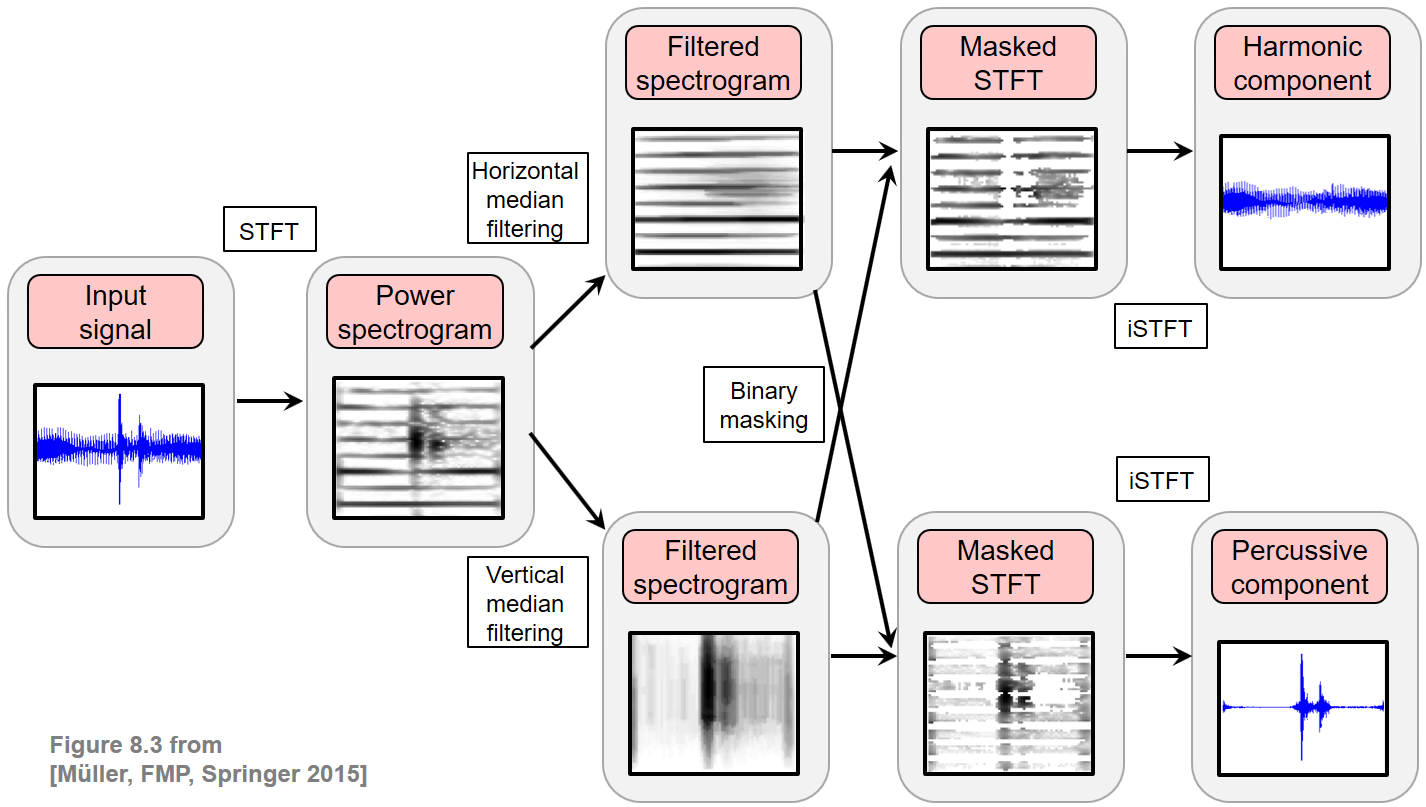
\includegraphics[width=0.8\textwidth]{figures/FMP_C8_F03.png}
\end{center}

\note[item]{For the purpose of this study, Fourier transform is a transform
whose input is a function and whose output is a complex valued function
of frequency. Typically, the input function represents a signal changing over
time or space. The output function maps a frequency to a complex number that
encapsulates the amplitude and phase of the wave. In other words, Fourier
transform breaks down a function into its constituent periodic functions.}
\note[item]{The Fourier transform is a integral over the whole real line. In the
context of the input being a signal over time, this means that the Fourier
transform cannot represent how the signal changes at each point in time. This is
where the short-time Fourier transform comes in. The STFT divides the input
signal into equal length, overlapping segments and applies the Fourier transform
to each of these segments. For a mathematical definition, the STFT is a
transform that takes a signal function and a window function and returns a
function of time and frequency, representing a wave at a point in time.}
\note[item]{In practice, many interesting signals are not stationary, meaning
they change over time. STFT can be used in these cases to extract richer data
about the input, which provides applications in musical and audio signal
analysis as well as in medical field for brain waves or cardiac signals. A STFT
can usually be visualized with a spectrogram, which is most often a heat map,
where x-axis represents time, y-axis represents the frequencies, and the colors
represent the strength of the frequencies.}
\note[item]{One of my favourite applications of STFT is in harmonic percussive 
source separation, where we want to decompose a given audio signal into two 
parts: one consisting of the harmonic and another of the percussive events.
Harmonic sounds are what we perceive as having pitch such as a melody, while
percussive sounds are leaning towards rhythms such as a clap or a click. In a
spectrogram, harmonic sounds are often characterized by a horizontal line as
they are more stationary over time, while percussive sounds are often vertical
lines as they are a burst across all frequencies at a single point in time. The
idea behind harmonic percussive source separation is to apply time-frequency
masks along horizontal and vertical directions to the spectrogram/STFT of an
input to get the harmonic and percussive sounds.}
\end{frame}

\begin{frame}
\frametitle{What are the parallel approaches to STFT?}
There are three families of STFT architecture designs \footcite{7419878}:
\begin{itemize}
    \item \textbf{FFT-based:} apply Fast Fourier Transform (FFT) to each segment
    \item \textbf{Iterative:} compute each segment from previous segment, new
    and discarded samples of the current segment
    \item \textbf{Feedforward:} reuse intermediate computations of the previous
    segment's FFT and compute only new samples
\end{itemize}
Software implmentations typically follow an FFT-based routine: apply a window
function to the input, execute FFT on a single segment, update result, then
repeat. Some level of parallelization is built-in but only targets the FFT
section.

\note[item]{To understand how STFTs are computed in practice, we can look at the
hardware designs. A study by Garrido categorized the designs into three groups.}
\note[item]{The first group, here we will refer to as FFT-based approach,
involves using several FFT modules in parallel. Each of these modules calculates
all the STFT frequencies at a certain time instant. We will go in more details
about FFT in a later section.}
\note[item]{The second group, namely the iterative approach, works on each
frequency, instead of each time point, in parallel. The values of each frequency
is computed iteratively by updating the value at a time point with an incoming
sample at the next time point.}
\note[item]{The third group will be referred to as the feedforward approach. It
calculates the Fourier transform of a segment by reusing the operations of
previous segments to avoid redundant computations.}
\note[item]{The reason why we are interested in hardware architectures is
because in software implmenetations, we do not observe such a variety in the
implementations of STFT. All of the popular libraries that we investigate,
including MATLAB, librosa, scipy, and torch, apply a similar approach to the
FFT-based design. These built-in routines obtain a signal frame from the input
using a specified window function, then compute a classical FFT on the signal
frame, and repeat for all frames of the input. There is some level of native
parallelization offered by these libraries, for example, MATLAB runs
multithreaded FFT and librosa uses vectorization. However, in general there is
limited work on different parallelization techniques software wise.}
\note[item]{We are taking the inspiration from the hardware designs and
implementing the software versions of the FFT-based and the feedforward
approaches. The iterative approach is out of scope, as it accumulates error over
time and makes it difficult to verify the correctness of the algorithm.}
\end{frame}

\begin{frame}
\frametitle{Why study STFT?}
\begin{itemize}
    \item Use cases for STFT span various research and practical fields.
    \item Parallel software implementations of STFT are not well studied and
    applied in common use, particularly so compared to Fourier transform.
\end{itemize}

\note[item]{In short, the motivation for this study can be summarized with the
following two points. First, we observe that STFT provides important information
distinct from those revealed by the classic Fourier transform, and these data
are widely applied in various fields. Second, study in STFT software
implementations, particularly their parallel approaches, is scarce relative to
that of Fourier transform. Commonly used mathematical and scientific libraries
offer limited implementations and generally do not allow user-level
configuration of parallelization.}
\end{frame}

\section{Methodology}
\begin{frame}
\frametitle{Which algorithms are compared?}
The study provides serial and parallel implementations, including
shared-memory, distributed-memory, and hybrid parallelization, of an FFT-based
algorithm and a feedforward algorithm. The code, together with collected results
and the visualization scripts used in this study are available on GitHub at 
https://github.com/chaunguyenm/stft. \footcite{stft-repo}.

\note[item]{The implementations in this study work on input signals where the
size of a segment is a power of 2, the window function is a rectangular window,
i.e., it simply takes a subarray of the input signal and does no other
modification, and the hop size or the distance between the beginning of two
consecutive segments is 1.}
\end{frame}

\begin{frame}
\frametitle{Serial FFT-based algorithm}
\begin{itemize}
    \item<1-> The algorithm uses a radix-2 decimation-in-time FFT implementation.
    \par \begin{tikzpicture}

% ============================================================
% Configuration
% ============================================================

\def\rowsep{0.5}

% ============================================================
% Helper macros
% ============================================================

% Stage nodes
%
% #1 = x position
% #2 = overlay specification
% #3 = node prefix
% #4 = fill
%
\newcommand{\drawstage}[4]{%
    \foreach \i in {0,...,7} {
        \node<#2>[
            circle,
            fill=#4,
            inner sep=0,
            minimum size=.1cm
        ] (#3\i) at (#1,-\i*\rowsep) {};
    }
}

% Variable box
%
% #1 = overlay
% #2 = node name
% #3 = x
% #4 = y
% #5 = label
% #6 = number of parts
% #7 = fill specification
% #8 = contents
%
\newcommand{\varbox}[8]{%
    \node<#1>[
        rectangle split,
        rectangle split horizontal,
        rectangle split parts=#6,
        draw,
        rectangle split part fill={#7},
        label=left:{#5}
    ] (#2) at (#3,#4) {#8};
}

% ============================================================
% Input
% ============================================================

\only<1>{
    \foreach \i in {0,...,7} {
        \node (x\i) at (0,-\i*\rowsep) {$x[\i]$};
    }
}

% ============================================================
% Bit-reversed input
%
% Original indices:
%
%   0 -> 0
%   1 -> 4
%   2 -> 2
%   3 -> 6
%   4 -> 1
%   5 -> 5
%   6 -> 3
%   7 -> 7
% ============================================================

\only<2->{
    \node (xr0) at (0,0)       {$x[0]$};
    \node (xr1) at (0,-0.5)    {$x[4]$};
    \node (xr2) at (0,-1)      {$x[2]$};
    \node (xr3) at (0,-1.5)    {$x[6]$};
    \node (xr4) at (0,-2)      {$x[1]$};
    \node (xr5) at (0,-2.5)    {$x[5]$};
    \node (xr6) at (0,-3)      {$x[3]$};
    \node (xr7) at (0,-3.5)    {$x[7]$};
}

% ============================================================
% FFT stages
% ============================================================

\drawstage{1}{2-}{s1s_}{black}
\drawstage{2}{3-}{s1e_}{white}

\drawstage{2.25}{7-}{s2s_}{black}
\drawstage{3.25}{8-}{s2e_}{white}

\drawstage{3.5}{12-}{s3s_}{black}
\drawstage{4.5}{13-}{s3e_}{white}

% ============================================================
% Starting connections
% ============================================================

\foreach \i in {0,...,7} {
    \draw<2->[-] (xr\i) -- (s1s_\i);
}
\foreach \i in {0,...,7} {
    \draw<7->[-] (s1e_\i) -- (s2s_\i);
}
\foreach \i in {0,...,7} {
    \draw<12->[-] (s2e_\i) -- (s3s_\i);
}

% ============================================================
% Stage 1: size = 2
% ============================================================

% ------------------------------------------------------------
% i = 0
% ------------------------------------------------------------

\varbox{3-3}{size}{7.5}{0}{size}{3}
    {gray!70,none,none}{
        \nodepart{one}$2$
        \nodepart{two}$4$
        \nodepart{three}$8$
    }

\varbox{3-3}{ivar}{7.5}{-0.5}{i}{8}
    {gray!70,none,none,none,none,none,none,none}{
        \nodepart{one}$0$
        \nodepart{two}$1$
        \nodepart{three}$2$
        \nodepart{four}$3$
        \nodepart{five}$4$
        \nodepart{six}$5$
        \nodepart{seven}$6$
        \nodepart{eight}$7$
    }

\varbox{3-3}{jvar}{7.5}{-1}{j}{1}{gray!70}{
    \nodepart{one}$0$
}

\varbox{3-3}{kvar}{7.5}{-1.5}{k}{1}{gray!70}{
    \nodepart{one}$0$
}

\varbox{3-3}{exp}{7.5}{-2.5}{exp}{4}
    {gray!70,none,none,none}{
        \nodepart{one}$W_8^0$
        \nodepart{two}$W_8^1$
        \nodepart{three}$W_8^2$
        \nodepart{four}$W_8^3$
    }

\draw<3->[-] (s1s_0) -- (s1e_0);
\draw<3->[-] (s1s_0) -- (s1e_1);
\draw<3->[-] (s1s_1) -- (s1e_0);
\draw<3->[-] (s1s_1) -- node[midway, below] {\tiny $-1$} (s1e_1);
\draw<3->[-] (xr1) -- node[midway, below] {\tiny $W_8^0$} (s1s_1);

\node<3->[circle, fill=black, inner sep=0, minimum size=.1cm] at (s1e_0) {};
\node<3->[circle, fill=black, inner sep=0, minimum size=.1cm] at (s1e_1) {};

% ------------------------------------------------------------
% i = 2
% ------------------------------------------------------------

\varbox{4-4}{size}{7.5}{0}{size}{3}
    {gray!70,none,none}{
        \nodepart{one}$2$
        \nodepart{two}$4$
        \nodepart{three}$8$
    }

\varbox{4-4}{ivar}{7.5}{-0.5}{i}{8}
    {none,none,gray!70,none,none,none,none,none}{
        \nodepart{one}$0$
        \nodepart{two}$1$
        \nodepart{three}$2$
        \nodepart{four}$3$
        \nodepart{five}$4$
        \nodepart{six}$5$
        \nodepart{seven}$6$
        \nodepart{eight}$7$
    }

\varbox{4-4}{jvar}{7.5}{-1}{j}{1}{gray!70}{
    \nodepart{one}$2$
}

\varbox{4-4}{kvar}{7.5}{-1.5}{k}{1}{gray!70}{
    \nodepart{one}$0$
}

\varbox{4-4}{exp}{7.5}{-2.5}{exp}{4}
    {gray!70,none,none,none}{
        \nodepart{one}$W_8^0$
        \nodepart{two}$W_8^1$
        \nodepart{three}$W_8^2$
        \nodepart{four}$W_8^3$
    }

\draw<4->[-] (s1s_2) -- (s1e_2);
\draw<4->[-] (s1s_2) -- (s1e_3);
\draw<4->[-] (s1s_3) -- (s1e_2);
\draw<4->[-] (s1s_3) -- node[midway, below] {\tiny $-1$} (s1e_3);
\draw<4->[-] (xr3) -- node[midway, below] {\tiny $W_8^0$} (s1s_3);

\node<4->[circle, fill=black, inner sep=0, minimum size=.1cm] at (s1e_2) {};
\node<4->[circle, fill=black, inner sep=0, minimum size=.1cm] at (s1e_3) {};

% ------------------------------------------------------------
% i = 4
% ------------------------------------------------------------

\varbox{5-5}{size}{7.5}{0}{size}{3}
    {gray!70,none,none}{
        \nodepart{one}$2$
        \nodepart{two}$4$
        \nodepart{three}$8$
    }

\varbox{5-5}{ivar}{7.5}{-0.5}{i}{8}
    {none,none,none,none,gray!70,none,none,none}{
        \nodepart{one}$0$
        \nodepart{two}$1$
        \nodepart{three}$2$
        \nodepart{four}$3$
        \nodepart{five}$4$
        \nodepart{six}$5$
        \nodepart{seven}$6$
        \nodepart{eight}$7$
    }

\varbox{5-5}{jvar}{7.5}{-1}{j}{1}{gray!70}{
    \nodepart{one}$4$
}

\varbox{5-5}{kvar}{7.5}{-1.5}{k}{1}{gray!70}{
    \nodepart{one}$0$
}

\varbox{5-5}{exp}{7.5}{-2.5}{exp}{4}
    {gray!70,none,none,none}{
        \nodepart{one}$W_8^0$
        \nodepart{two}$W_8^1$
        \nodepart{three}$W_8^2$
        \nodepart{four}$W_8^3$
    }

\draw<5->[-] (s1s_4) -- (s1e_4);
\draw<5->[-] (s1s_4) -- (s1e_5);
\draw<5->[-] (s1s_5) -- (s1e_4);
\draw<5->[-] (s1s_5) -- node[midway, below] {\tiny $-1$} (s1e_5);
\draw<5->[-] (xr5) -- node[midway, below] {\tiny $W_8^0$} (s1s_5);

\node<5->[circle, fill=black, inner sep=0, minimum size=.1cm] at (s1e_4) {};
\node<5->[circle, fill=black, inner sep=0, minimum size=.1cm] at (s1e_5) {};

% ------------------------------------------------------------
% i = 6
% ------------------------------------------------------------

\varbox{6-6}{size}{7.5}{0}{size}{3}
    {gray!70,none,none}{
        \nodepart{one}$2$
        \nodepart{two}$4$
        \nodepart{three}$8$
    }

\varbox{6-6}{ivar}{7.5}{-0.5}{i}{8}
    {none,none,none,none,none,none,gray!70,none}{
        \nodepart{one}$0$
        \nodepart{two}$1$
        \nodepart{three}$2$
        \nodepart{four}$3$
        \nodepart{five}$4$
        \nodepart{six}$5$
        \nodepart{seven}$6$
        \nodepart{eight}$7$
    }

\varbox{6-6}{jvar}{7.5}{-1}{j}{1}{gray!70}{
    \nodepart{one}$6$
}

\varbox{6-6}{kvar}{7.5}{-1.5}{k}{1}{gray!70}{
    \nodepart{one}$0$
}

\varbox{6-6}{exp}{7.5}{-2.5}{exp}{4}
    {gray!70,none,none,none}{
        \nodepart{one}$W_8^0$
        \nodepart{two}$W_8^1$
        \nodepart{three}$W_8^2$
        \nodepart{four}$W_8^3$
    }

\draw<6->[-] (s1s_6) -- (s1e_6);
\draw<6->[-] (s1s_6) -- (s1e_7);
\draw<6->[-] (s1s_7) -- (s1e_6);
\draw<6->[-] (s1s_7) -- node[midway, below] {\tiny $-1$} (s1e_7);
\draw<6->[-] (xr7) -- node[midway, below] {\tiny $W_8^0$} (s1s_7);

\node<6->[circle, fill=black, inner sep=0, minimum size=.1cm] at (s1e_6) {};
\node<6->[circle, fill=black, inner sep=0, minimum size=.1cm] at (s1e_7) {};

% ============================================================
% Stage 2: size = 4
% ============================================================

% ------------------------------------------------------------
% i = 0, j = 0
% ------------------------------------------------------------

\varbox{8-8}{size}{7.5}{0}{size}{3}
    {none,gray!70,none}{
        \nodepart{one}$2$
        \nodepart{two}$4$
        \nodepart{three}$8$
    }

\varbox{8-8}{ivar}{7.5}{-0.5}{i}{8}
    {gray!70,none,none,none,none,none,none,none}{
        \nodepart{one}$0$
        \nodepart{two}$1$
        \nodepart{three}$2$
        \nodepart{four}$3$
        \nodepart{five}$4$
        \nodepart{six}$5$
        \nodepart{seven}$6$
        \nodepart{eight}$7$
    }

\varbox{8-8}{jvar}{7.5}{-1}{j}{2}{gray!70,none}{
    \nodepart{one}$0$
    \nodepart{two}$1$
}

\varbox{8-8}{kvar}{7.5}{-1.5}{k}{2}{gray!70, none}{
    \nodepart{one}$0$
    \nodepart{two}$2$
}

\varbox{8-8}{exp}{7.5}{-2.5}{exp}{4}
    {gray!70,none,none,none}{
        \nodepart{one}$W_8^0$
        \nodepart{two}$W_8^1$
        \nodepart{three}$W_8^2$
        \nodepart{four}$W_8^3$
    }

\draw<8->[-] (s2s_0) -- (s2e_0);
\draw<8->[-] (s2s_0) -- (s2e_2);
\draw<8->[-] (s2s_2) -- (s2e_0);
\draw<8->[-] (s2s_2) -- node[midway, below] {\tiny $-1$} (s2e_2);
\draw<8->[-] (s1e_2) -- node[midway, below] {\tiny $W_8^0$} (s2s_2);

\node<8->[circle, fill=black, inner sep=0, minimum size=.1cm] at (s2e_0) {};
\node<8->[circle, fill=black, inner sep=0, minimum size=.1cm] at (s2e_2) {};

% ============================================================
% Stage 2: size = 4
% ============================================================

% ------------------------------------------------------------
% i = 0, j = 2
% ------------------------------------------------------------

\varbox{9-9}{size}{7.5}{0}{size}{3}
    {none,gray!70,none}{
        \nodepart{one}$2$
        \nodepart{two}$4$
        \nodepart{three}$8$
    }

\varbox{9-9}{ivar}{7.5}{-0.5}{i}{8}
    {gray!70,none,none,none,none,none,none,none}{
        \nodepart{one}$0$
        \nodepart{two}$1$
        \nodepart{three}$2$
        \nodepart{four}$3$
        \nodepart{five}$4$
        \nodepart{six}$5$
        \nodepart{seven}$6$
        \nodepart{eight}$7$
    }

\varbox{9-9}{jvar}{7.5}{-1}{j}{2}{none,gray!70}{
    \nodepart{one}$0$
    \nodepart{two}$1$
}

\varbox{9-9}{kvar}{7.5}{-1.5}{k}{2}{none,gray!70}{
    \nodepart{one}$0$
    \nodepart{two}$2$
}

\varbox{9-9}{exp}{7.5}{-2.5}{exp}{4}
    {none,none,gray!70,none}{
        \nodepart{one}$W_8^0$
        \nodepart{two}$W_8^1$
        \nodepart{three}$W_8^2$
        \nodepart{four}$W_8^3$
    }

\draw<9->[-] (s2s_1) -- (s2e_1);
\draw<9->[-] (s2s_1) -- (s2e_3);
\draw<9->[-] (s2s_3) -- (s2e_1);
\draw<9->[-] (s2s_3) -- node[midway, below] {\tiny $-1$} (s2e_3);
\draw<9->[-] (s1e_3) -- node[midway, below] {\tiny $W_8^2$} (s2s_3);

\node<9->[circle, fill=black, inner sep=0, minimum size=.1cm] at (s2e_1) {};
\node<9->[circle, fill=black, inner sep=0, minimum size=.1cm] at (s2e_3) {};

% ============================================================
% Stage 2: size = 4
% ============================================================

% ------------------------------------------------------------
% i = 4, j = 4
% ------------------------------------------------------------

\varbox{10-10}{size}{7.5}{0}{size}{3}
    {none,gray!70,none}{
        \nodepart{one}$2$
        \nodepart{two}$4$
        \nodepart{three}$8$
    }

\varbox{10-10}{ivar}{7.5}{-0.5}{i}{8}
    {none,none,none,none,gray!70,none,none,none}{
        \nodepart{one}$0$
        \nodepart{two}$1$
        \nodepart{three}$2$
        \nodepart{four}$3$
        \nodepart{five}$4$
        \nodepart{six}$5$
        \nodepart{seven}$6$
        \nodepart{eight}$7$
    }

\varbox{10-10}{jvar}{7.5}{-1}{j}{2}{gray!70,none}{
    \nodepart{one}$4$
    \nodepart{two}$5$
}

\varbox{10-10}{kvar}{7.5}{-1.5}{k}{2}{gray!70,none}{
    \nodepart{one}$0$
    \nodepart{two}$2$
}

\varbox{10-10}{exp}{7.5}{-2.5}{exp}{4}
    {gray!70,none,none,none}{
        \nodepart{one}$W_8^0$
        \nodepart{two}$W_8^1$
        \nodepart{three}$W_8^2$
        \nodepart{four}$W_8^3$
    }

\draw<10->[-] (s2s_4) -- (s2e_4);
\draw<10->[-] (s2s_4) -- (s2e_6);
\draw<10->[-] (s2s_6) -- (s2e_4);
\draw<10->[-] (s2s_6) -- node[midway, below] {\tiny $-1$} (s2e_6);
\draw<10->[-] (s1e_6) -- node[midway, below] {\tiny $W_8^0$} (s2s_6);

\node<10->[circle, fill=black, inner sep=0, minimum size=.1cm] at (s2e_4) {};
\node<10->[circle, fill=black, inner sep=0, minimum size=.1cm] at (s2e_6) {};

% ============================================================
% Stage 2: size = 4
% ============================================================

% ------------------------------------------------------------
% i = 4, j = 5
% ------------------------------------------------------------

\varbox{11-11}{size}{7.5}{0}{size}{3}
    {none,gray!70,none}{
        \nodepart{one}$2$
        \nodepart{two}$4$
        \nodepart{three}$8$
    }

\varbox{11-11}{ivar}{7.5}{-0.5}{i}{8}
    {none,none,none,none,gray!70,none,none,none}{
        \nodepart{one}$0$
        \nodepart{two}$1$
        \nodepart{three}$2$
        \nodepart{four}$3$
        \nodepart{five}$4$
        \nodepart{six}$5$
        \nodepart{seven}$6$
        \nodepart{eight}$7$
    }

\varbox{11-11}{jvar}{7.5}{-1}{j}{2}{none,gray!70}{
    \nodepart{one}$4$
    \nodepart{two}$5$
}

\varbox{11-11}{kvar}{7.5}{-1.5}{k}{2}{none,gray!70}{
    \nodepart{one}$0$
    \nodepart{two}$2$
}

\varbox{11-11}{exp}{7.5}{-2.5}{exp}{4}
    {none,none,gray!70,none}{
        \nodepart{one}$W_8^0$
        \nodepart{two}$W_8^1$
        \nodepart{three}$W_8^2$
        \nodepart{four}$W_8^3$
    }

\draw<11->[-] (s2s_5) -- (s2e_5);
\draw<11->[-] (s2s_5) -- (s2e_7);
\draw<11->[-] (s2s_7) -- (s2e_5);
\draw<11->[-] (s2s_7) -- node[midway, below] {\tiny $-1$} (s2e_7);
\draw<11->[-] (s1e_7) -- node[midway, below] {\tiny $W_8^2$} (s2s_7);

\node<11->[circle, fill=black, inner sep=0, minimum size=.1cm] at (s2e_5) {};
\node<11->[circle, fill=black, inner sep=0, minimum size=.1cm] at (s2e_7) {};

% ============================================================
% Stage 3: size = 8
% ============================================================

% ------------------------------------------------------------
% i = 0, j = 0
% ------------------------------------------------------------

\varbox{13-13}{size}{7.5}{0}{size}{3}
    {none,none,gray!70}{
        \nodepart{one}$2$
        \nodepart{two}$4$
        \nodepart{three}$8$
    }

\varbox{13-13}{ivar}{7.5}{-0.5}{i}{8}
    {gray!70,none,none,none,none,none,none,none}{
        \nodepart{one}$0$
        \nodepart{two}$1$
        \nodepart{three}$2$
        \nodepart{four}$3$
        \nodepart{five}$4$
        \nodepart{six}$5$
        \nodepart{seven}$6$
        \nodepart{eight}$7$
    }

\varbox{13-13}{jvar}{7.5}{-1}{j}{4}{gray!70,none,none,none}{
    \nodepart{one}$0$
    \nodepart{two}$1$
    \nodepart{three}$2$
    \nodepart{four}$3$
}

\varbox{13-13}{kvar}{7.5}{-1.5}{k}{4}{gray!70,none,none,none}{
    \nodepart{one}$0$
    \nodepart{two}$1$
    \nodepart{three}$2$
    \nodepart{four}$3$
}

\varbox{13-13}{exp}{7.5}{-2.5}{exp}{4}
    {gray!70,none,none,none}{
        \nodepart{one}$W_8^0$
        \nodepart{two}$W_8^1$
        \nodepart{three}$W_8^2$
        \nodepart{four}$W_8^3$
    }

\draw<13->[-] (s3s_0) -- (s3e_0);
\draw<13->[-] (s3s_0) -- (s3e_4);
\draw<13->[-] (s3s_4) -- (s3e_0);
\draw<13->[-] (s3s_4) -- node[midway, below] {\tiny $-1$} (s3e_4);
\draw<13->[-] (s2e_4) -- node[midway, below] {\tiny $W_8^0$} (s3s_4);

\node<13->[circle, fill=black, inner sep=0, minimum size=.1cm] at (s3e_0) {};
\node<13->[circle, fill=black, inner sep=0, minimum size=.1cm] at (s3e_4) {};

% ============================================================
% Stage 3: size = 8
% ============================================================

% ------------------------------------------------------------
% i = 0, j = 1
% ------------------------------------------------------------

\varbox{14-14}{size}{7.5}{0}{size}{3}
    {none,none,gray!70}{
        \nodepart{one}$2$
        \nodepart{two}$4$
        \nodepart{three}$8$
    }

\varbox{14-14}{ivar}{7.5}{-0.5}{i}{8}
    {gray!70,none,none,none,none,none,none,none}{
        \nodepart{one}$0$
        \nodepart{two}$1$
        \nodepart{three}$2$
        \nodepart{four}$3$
        \nodepart{five}$4$
        \nodepart{six}$5$
        \nodepart{seven}$6$
        \nodepart{eight}$7$
    }

\varbox{14-14}{jvar}{7.5}{-1}{j}{4}{none,gray!70,none,none}{
    \nodepart{one}$0$
    \nodepart{two}$1$
    \nodepart{three}$2$
    \nodepart{four}$3$
}

\varbox{14-14}{kvar}{7.5}{-1.5}{k}{4}{none,gray!70,none,none}{
    \nodepart{one}$0$
    \nodepart{two}$1$
    \nodepart{three}$2$
    \nodepart{four}$3$
}

\varbox{14-14}{exp}{7.5}{-2.5}{exp}{4}
    {none,gray!70,none,none}{
        \nodepart{one}$W_8^0$
        \nodepart{two}$W_8^1$
        \nodepart{three}$W_8^2$
        \nodepart{four}$W_8^3$
    }

\draw<14->[-] (s3s_1) -- (s3e_1);
\draw<14->[-] (s3s_1) -- (s3e_5);
\draw<14->[-] (s3s_5) -- (s3e_1);
\draw<14->[-] (s3s_5) -- node[midway, below] {\tiny $-1$} (s3e_5);
\draw<14->[-] (s2e_5) -- node[midway, below] {\tiny $W_8^1$} (s3s_5);

\node<14->[circle, fill=black, inner sep=0, minimum size=.1cm] at (s3e_1) {};
\node<14->[circle, fill=black, inner sep=0, minimum size=.1cm] at (s3e_5) {};

% ============================================================
% Stage 3: size = 8
% ============================================================

% ------------------------------------------------------------
% i = 0, j = 2
% ------------------------------------------------------------

\varbox{15-15}{size}{7.5}{0}{size}{3}
    {none,none,gray!70}{
        \nodepart{one}$2$
        \nodepart{two}$4$
        \nodepart{three}$8$
    }

\varbox{15-15}{ivar}{7.5}{-0.5}{i}{8}
    {gray!70,none,none,none,none,none,none,none}{
        \nodepart{one}$0$
        \nodepart{two}$1$
        \nodepart{three}$2$
        \nodepart{four}$3$
        \nodepart{five}$4$
        \nodepart{six}$5$
        \nodepart{seven}$6$
        \nodepart{eight}$7$
    }

\varbox{15-15}{jvar}{7.5}{-1}{j}{4}{none,none,gray!70,none}{
    \nodepart{one}$0$
    \nodepart{two}$1$
    \nodepart{three}$2$
    \nodepart{four}$3$
}

\varbox{15-15}{kvar}{7.5}{-1.5}{k}{4}{none,none,gray!70,none}{
    \nodepart{one}$0$
    \nodepart{two}$1$
    \nodepart{three}$2$
    \nodepart{four}$3$
}

\varbox{15-15}{exp}{7.5}{-2.5}{exp}{4}
    {none,none,gray!70,none}{
        \nodepart{one}$W_8^0$
        \nodepart{two}$W_8^1$
        \nodepart{three}$W_8^2$
        \nodepart{four}$W_8^3$
    }

\draw<15->[-] (s3s_2) -- (s3e_2);
\draw<15->[-] (s3s_2) -- (s3e_6);
\draw<15->[-] (s3s_6) -- (s3e_2);
\draw<15->[-] (s3s_6) -- node[midway, below] {\tiny $-1$} (s3e_6);
\draw<15->[-] (s2e_6) -- node[midway, below] {\tiny $W_8^2$} (s3s_6);

\node<15->[circle, fill=black, inner sep=0, minimum size=.1cm] at (s3e_2) {};
\node<15->[circle, fill=black, inner sep=0, minimum size=.1cm] at (s3e_6) {};

% ============================================================
% Stage 3: size = 8
% ============================================================

% ------------------------------------------------------------
% i = 0, j = 3
% ------------------------------------------------------------

\varbox{16-16}{size}{7.5}{0}{size}{3}
    {none,none,gray!70}{
        \nodepart{one}$2$
        \nodepart{two}$4$
        \nodepart{three}$8$
    }

\varbox{16-16}{ivar}{7.5}{-0.5}{i}{8}
    {gray!70,none,none,none,none,none,none,none}{
        \nodepart{one}$0$
        \nodepart{two}$1$
        \nodepart{three}$2$
        \nodepart{four}$3$
        \nodepart{five}$4$
        \nodepart{six}$5$
        \nodepart{seven}$6$
        \nodepart{eight}$7$
    }

\varbox{16-16}{jvar}{7.5}{-1}{j}{4}{none,none,none,gray!70}{
    \nodepart{one}$0$
    \nodepart{two}$1$
    \nodepart{three}$2$
    \nodepart{four}$3$
}

\varbox{16-16}{kvar}{7.5}{-1.5}{k}{4}{none,none,none,gray!70}{
    \nodepart{one}$0$
    \nodepart{two}$1$
    \nodepart{three}$2$
    \nodepart{four}$3$
}

\varbox{16-16}{exp}{7.5}{-2.5}{exp}{4}
    {none,none,none,gray!70}{
        \nodepart{one}$W_8^0$
        \nodepart{two}$W_8^1$
        \nodepart{three}$W_8^2$
        \nodepart{four}$W_8^3$
    }

\draw<16->[-] (s3s_3) -- (s3e_3);
\draw<16->[-] (s3s_3) -- (s3e_7);
\draw<16->[-] (s3s_7) -- (s3e_3);
\draw<16->[-] (s3s_7) -- node[midway, below] {\tiny $-1$} (s3e_7);
\draw<16->[-] (s2e_7) -- node[midway, below] {\tiny $W_8^3$} (s3s_7);

\node<16->[circle, fill=black, inner sep=0, minimum size=.1cm] at (s3e_3) {};
\node<16->[circle, fill=black, inner sep=0, minimum size=.1cm] at (s3e_7) {};

% ============================================================
% Output
% ============================================================

\foreach \i in {0,...,7} {
    \node<17-> (X\i) at (5.5,-\i*\rowsep) {$X[\i]$};
}
\foreach \i in {0,...,7} {
    \draw<17->[-] (s3e_\i) -- (X\i);
}

\end{tikzpicture}

    \item<18-> The algorithm applies FFT to each segment in order.
    \par 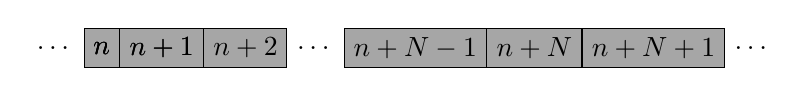
\begin{tikzpicture}
    \node[anchor=west] (d1) at (0,0) {\dots};
    \node[
        anchor=west,
        rectangle split,
        rectangle split horizontal,
        rectangle split parts=3,
        draw,
        rectangle split part fill=none,
    ] (input1) at (d1.east) {
        \nodepart{one}$n$
        \nodepart{two}$n+1$
        \nodepart{three}$n+2$
    };

    \node[anchor=west] (d2) at (input1.east) {\dots};
    \node[
        anchor=west,
        rectangle split,
        rectangle split horizontal,
        rectangle split parts=3,
        draw,
        rectangle split part fill=none,
    ] (input2) at (d2.east) {
        \nodepart{one}$n+N-1$
        \nodepart{two}$n+N$
        \nodepart{three}$n+N+1$
    };

    \node[anchor=west] (d3) at (input2.east) {\dots};

    % ------------------------------------------------------------
    % Highlight
    % ------------------------------------------------------------

    % 1st FFT
    \node<19-19>[
        anchor=west,
        rectangle split,
        rectangle split horizontal,
        rectangle split parts=3,
        draw,
        rectangle split part fill=gray!70,
    ] (input1) at (d1.east) {
        \nodepart{one}$n$
        \nodepart{two}$n+1$
        \nodepart{three}$n+2$
    };
    \node<19-19>[
        anchor=west,
        rectangle split,
        rectangle split horizontal,
        rectangle split parts=3,
        draw,
        rectangle split part fill={gray!70,none,none},
    ] (input2) at (d2.east) {
        \nodepart{one}$n+N-1$
        \nodepart{two}$n+N$
        \nodepart{three}$n+N+1$
    };

    % 2nd FFT
    \node<20-20>[
        anchor=west,
        rectangle split,
        rectangle split horizontal,
        rectangle split parts=3,
        draw,
        rectangle split part fill={none,gray!70,gray!70},
    ] (input1) at (d1.east) {
        \nodepart{one}$n$
        \nodepart{two}$n+1$
        \nodepart{three}$n+2$
    };
    \node<20-20>[
        anchor=west,
        rectangle split,
        rectangle split horizontal,
        rectangle split parts=3,
        draw,
        rectangle split part fill={gray!70,gray!70,none},
    ] (input2) at (d2.east) {
        \nodepart{one}$n+N-1$
        \nodepart{two}$n+N$
        \nodepart{three}$n+N+1$
    };

    % 3rd FFT
    \node<21-21>[
        anchor=west,
        rectangle split,
        rectangle split horizontal,
        rectangle split parts=3,
        draw,
        rectangle split part fill={none,none,gray!70},
    ] (input1) at (d1.east) {
        \nodepart{one}$n$
        \nodepart{two}$n+1$
        \nodepart{three}$n+2$
    };
    \node<21-21>[
        anchor=west,
        rectangle split,
        rectangle split horizontal,
        rectangle split parts=3,
        draw,
        rectangle split part fill=gray!70,
    ] (input2) at (d2.east) {
        \nodepart{one}$n+N-1$
        \nodepart{two}$n+N$
        \nodepart{three}$n+N+1$
    };
\end{tikzpicture}

\end{itemize}

\note[item]{For the serial FFT-based algorithm of STFT, this study uses a 
standard radix-2 decimation-in-time FFT implementation. For those who are not
familiar with FFT, it is an efficient algorithm to compute the discrete Fourier
transform, reducing the number of computations needed from N squared to NlogN. It does
this by taking advantage of the symmetry in the calculation of the transform and
using a divide-and-conquer method. In the ideal scenario where the number of
samples in the input signal, referred to as big N, is a power of 2, the input is
split into even- and odd-indexed samples, and the transform is calculated on
each of these smaller sequences before being combined to obtain the final
result. Radix-2 here means we are assuming this ideal scenario of N being a
perfect power of 2, and decimation-in-time means input samples are being
rearranged in bit reversal order before calculating the transform, as opposed to
decimation in frequency where the transform is calculated first then the result
is rearranged.}
\note[item]{The FFT implementation in this study uses a breadth-first traversal
of the computational tree instead of the recursive divide-and-conquer method.
The algorithm first does a bit reversal rearrangement of the input signal. Bit
reversal is how the odd- and even-indexed signal samples are rearranged, where
the index of a sample is represented in binary and then flipped so that the the
most significant bit becomes the least significant. Then the algorithm builds 
out the twiddle factor table, and iterates through each computational stage, 
represented here as a different size. The operations can be visualized as shown,
and the diagram obtained after the last stage is typically called a butterfly 
diagram.}
\note[item]{The serial implementation of the FFT-based STFT will apply the FFT
algorithm described above to every segment of the input in order. In other
words, it iterates through the input signal, takes the effective segment, and
computes the discrete Fourier transform using the FFT algorithm, then combines
the results.}
\end{frame}

\begin{frame}
\frametitle{Parallel FFT-based algorithm}
\begin{itemize}
    \item Shared-memory: Multiple threads apply FFTs to segments in parallel.
    \item Distributed-memory: Multiple processes apply FFTs to an assigned
    subarray and \texttt{MPI\_Send} to one process.
\end{itemize}
\begin{center}
    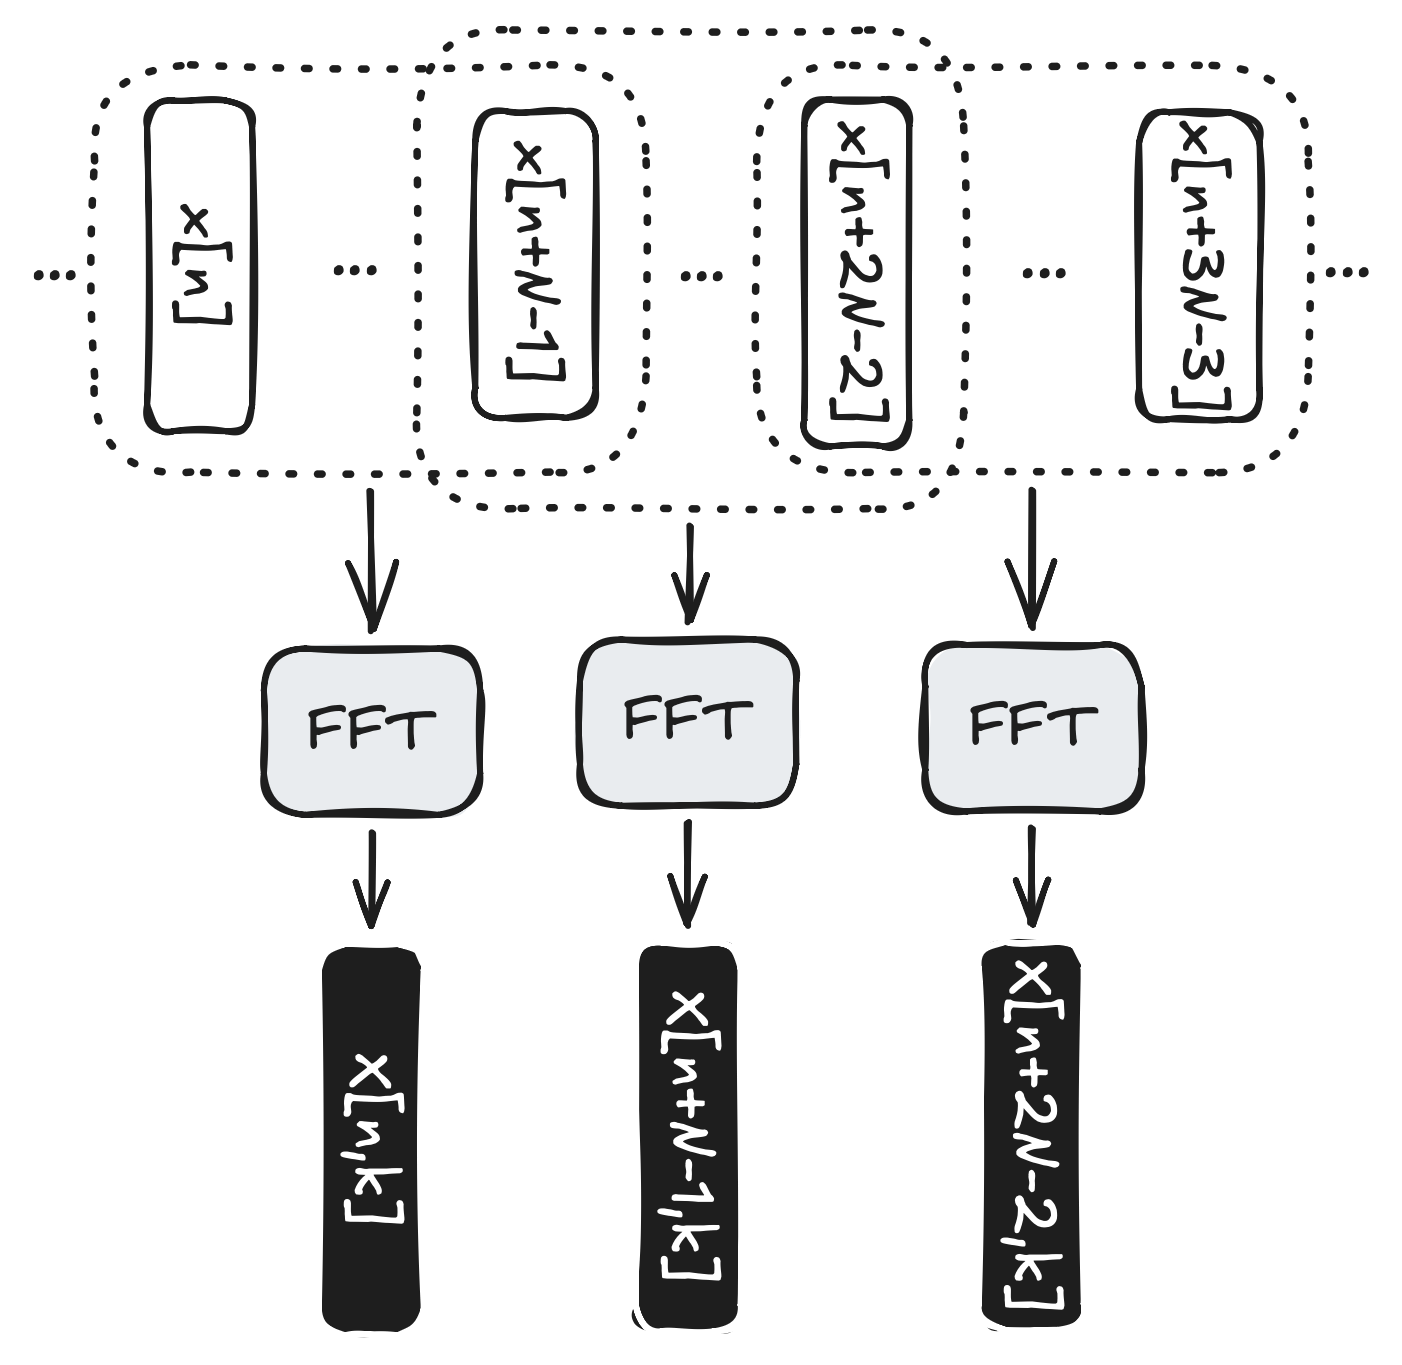
\includegraphics[width=0.5\textwidth]{figures/parallel-fft}
\end{center}

\note[item]{With OpenMP, the FFT-based short-time Fourier transform algorithm 
can perform FFT on each subarray and write the result to the final array in
parallel.}
\note[item]{The number of Fourier transforms are as evenly distributed as 
possible across all processes. Each process extracts the subarrays whose 
Fourier transforms it must compute, processes the computation using FFT then 
sends the results to the root process. Rank 0 is responsible for receiving from
each of the remaining processes and writes to the correct index of the returned
array.}
\end{frame}

\begin{frame}
\frametitle{Serial feedforward algorithm}
\textbf{Idea:} Reuse computations of the previous FFT and only incur
computations involving new input. \footcite{7419878}
% ============================================================
% 8-point radix-2 DIT FFT diagram
%
% Usage:
%   \fft{0}
%   \fft{8}
%   \fft{16}
%
% The argument is the first input/output index.
% ============================================================

\newcommand{\fft}[3]{%
% \begin{tikzpicture}[scale=0.5]

% Store the first index
\pgfmathtruncatemacro{\base}{#1}
\pgfmathtruncatemacro{\xpos}{#2}
\pgfmathtruncatemacro{\ypos}{#3}

% ------------------------------------------------------------
% Input labels (bit-reversed order)
% ------------------------------------------------------------

\foreach \i/\v in {
    0/0,
    1/4,
    2/2,
    3/6,
    4/1,
    5/5,
    6/3,
    7/7
}{
    \pgfmathtruncatemacro{\idx}{\base+\v}
    \node (fft-\base-x-\i) at (0+\xpos,-\i+\ypos)
        {$x[\idx]$};
}

% ------------------------------------------------------------
% Stage nodes
% ------------------------------------------------------------

\foreach \i in {0,...,7}{
    \node[
        circle,
        fill=gray!70,
        inner sep=0,
        minimum size=.1cm
    ] (fft-\base-s0-\i) at (1+\xpos,-\i+\ypos) {};

    \node[
        circle,
        fill=gray!70,
        inner sep=0,
        minimum size=.1cm
    ] (fft-\base-s1-\i) at (2+\xpos,-\i+\ypos) {};

    \node[
        circle,
        fill=gray!70,
        inner sep=0,
        minimum size=.1cm
    ] (fft-\base-s2-\i) at (3+\xpos,-\i+\ypos) {};

    \node[
        circle,
        fill=gray!70,
        inner sep=0,
        minimum size=.1cm
    ] (fft-\base-s3-\i) at (4+\xpos,-\i+\ypos) {};
}

% ------------------------------------------------------------
% Input -> Stage 0
% ------------------------------------------------------------

% \foreach \i in {0,...,7}{
%     \draw[draw=gray!70]
%         (fft-\base-x-\i)
%         -- (fft-\base-s0-\i);
% }

% ------------------------------------------------------------
% Stage 1: butterflies of size 2
% ------------------------------------------------------------

\draw[draw=gray!70] (fft-\base-s0-0) -- (fft-\base-s1-0);
\draw[draw=gray!70] (fft-\base-s0-0) -- (fft-\base-s1-1);
\draw[draw=gray!70] (fft-\base-s0-1) -- (fft-\base-s1-0);
\draw[draw=gray!70] (fft-\base-s0-1) -- (fft-\base-s1-1);

\draw[draw=gray!70] (fft-\base-s0-2) -- (fft-\base-s1-2);
\draw[draw=gray!70] (fft-\base-s0-2) -- (fft-\base-s1-3);
\draw[draw=gray!70] (fft-\base-s0-3) -- (fft-\base-s1-2);
\draw[draw=gray!70] (fft-\base-s0-3) -- (fft-\base-s1-3);

\draw[draw=gray!70] (fft-\base-s0-4) -- (fft-\base-s1-4);
\draw[draw=gray!70] (fft-\base-s0-4) -- (fft-\base-s1-5);
\draw[draw=gray!70] (fft-\base-s0-5) -- (fft-\base-s1-4);
\draw[draw=gray!70] (fft-\base-s0-5) -- (fft-\base-s1-5);

\draw[draw=gray!70] (fft-\base-s0-6) -- (fft-\base-s1-6);
\draw[draw=gray!70] (fft-\base-s0-6) -- (fft-\base-s1-7);
\draw[draw=gray!70] (fft-\base-s0-7) -- (fft-\base-s1-6);
\draw[draw=gray!70] (fft-\base-s0-7) -- (fft-\base-s1-7);

% ------------------------------------------------------------
% Stage 2: butterflies of size 4
% ------------------------------------------------------------

\draw[draw=gray!70] (fft-\base-s1-0) -- (fft-\base-s2-0);
\draw[draw=gray!70] (fft-\base-s1-0) -- (fft-\base-s2-2);
\draw[draw=gray!70] (fft-\base-s1-2) -- (fft-\base-s2-0);
\draw[draw=gray!70] (fft-\base-s1-2) -- (fft-\base-s2-2);

\draw[draw=gray!70] (fft-\base-s1-1) -- (fft-\base-s2-1);
\draw[draw=gray!70] (fft-\base-s1-1) -- (fft-\base-s2-3);
\draw[draw=gray!70] (fft-\base-s1-3) -- (fft-\base-s2-1);
\draw[draw=gray!70] (fft-\base-s1-3) -- (fft-\base-s2-3);

\draw[draw=gray!70] (fft-\base-s1-4) -- (fft-\base-s2-4);
\draw[draw=gray!70] (fft-\base-s1-4) -- (fft-\base-s2-6);
\draw[draw=gray!70] (fft-\base-s1-6) -- (fft-\base-s2-4);
\draw[draw=gray!70] (fft-\base-s1-6) -- (fft-\base-s2-6);

\draw[draw=gray!70] (fft-\base-s1-5) -- (fft-\base-s2-5);
\draw[draw=gray!70] (fft-\base-s1-5) -- (fft-\base-s2-7);
\draw[draw=gray!70] (fft-\base-s1-7) -- (fft-\base-s2-5);
\draw[draw=gray!70] (fft-\base-s1-7) -- (fft-\base-s2-7);

% ------------------------------------------------------------
% Stage 3: butterflies of size 8
% ------------------------------------------------------------

\draw[draw=gray!70] (fft-\base-s2-0) -- (fft-\base-s3-0);
\draw[draw=gray!70] (fft-\base-s2-0) -- (fft-\base-s3-4);
\draw[draw=gray!70] (fft-\base-s2-4) -- (fft-\base-s3-0);
\draw[draw=gray!70] (fft-\base-s2-4) -- (fft-\base-s3-4);

\draw[draw=gray!70] (fft-\base-s2-1) -- (fft-\base-s3-1);
\draw[draw=gray!70] (fft-\base-s2-1) -- (fft-\base-s3-5);
\draw[draw=gray!70] (fft-\base-s2-5) -- (fft-\base-s3-1);
\draw[draw=gray!70] (fft-\base-s2-5) -- (fft-\base-s3-5);

\draw[draw=gray!70] (fft-\base-s2-2) -- (fft-\base-s3-2);
\draw[draw=gray!70] (fft-\base-s2-2) -- (fft-\base-s3-6);
\draw[draw=gray!70] (fft-\base-s2-6) -- (fft-\base-s3-2);
\draw[draw=gray!70] (fft-\base-s2-6) -- (fft-\base-s3-6);

\draw[draw=gray!70] (fft-\base-s2-3) -- (fft-\base-s3-3);
\draw[draw=gray!70] (fft-\base-s2-3) -- (fft-\base-s3-7);
\draw[draw=gray!70] (fft-\base-s2-7) -- (fft-\base-s3-3);
\draw[draw=gray!70] (fft-\base-s2-7) -- (fft-\base-s3-7);

% ------------------------------------------------------------
% Output labels
% ------------------------------------------------------------

\foreach \i in {0,...,7}{
    \pgfmathtruncatemacro{\idx}{\base+\i}
    \node (fft-\base-X-\i) at (5+\xpos,-\i+\ypos)
        {$X[\idx]$};
}

% ------------------------------------------------------------
% Stage 3 -> Output
% ------------------------------------------------------------

% \foreach \i in {0,...,7}{
%     \draw[draw=gray!70]
%         (fft-\base-s3-\i)
%         -- (fft-\base-X-\i);
% }

% \end{tikzpicture}
}

\begin{tikzpicture}[scale=0.5]
    \fft{0}{0}{0}
    \fft{1}{7}{0}
    \fft{2}{14}{0}

    % ------------------------------------------------------------
    % base0 vs base1
    % ------------------------------------------------------------

    \node<2-5>[circle, fill=black, inner sep=0, minimum size=.1cm] at (fft-0-s1-2) {};
    \node<2-5>[circle, fill=black, inner sep=0, minimum size=.1cm] at (fft-0-s1-3) {};
    \node<2-5>[circle, fill=black, inner sep=0, minimum size=.1cm] at (fft-1-s1-4) {};
    \node<2-5>[circle, fill=black, inner sep=0, minimum size=.1cm] at (fft-1-s1-5) {};

    \node<3-5>[circle, fill=black, inner sep=0, minimum size=.1cm] at (fft-0-s1-4) {};
    \node<3-5>[circle, fill=black, inner sep=0, minimum size=.1cm] at (fft-0-s1-5) {};
    \node<3-5>[circle, fill=black, inner sep=0, minimum size=.1cm] at (fft-1-s1-0) {};
    \node<3-5>[circle, fill=black, inner sep=0, minimum size=.1cm] at (fft-1-s1-1) {};
    
    \node<4-5>[circle, fill=black, inner sep=0, minimum size=.1cm] at (fft-0-s1-6) {};
    \node<4-5>[circle, fill=black, inner sep=0, minimum size=.1cm] at (fft-0-s1-7) {};
    \node<4-5>[circle, fill=black, inner sep=0, minimum size=.1cm] at (fft-1-s1-2) {};
    \node<4-5>[circle, fill=black, inner sep=0, minimum size=.1cm] at (fft-1-s1-3) {};
    
    \node<5-5>[circle, fill=black, inner sep=0, minimum size=.1cm] at (fft-0-s2-4) {};
    \node<5-5>[circle, fill=black, inner sep=0, minimum size=.1cm] at (fft-0-s2-5) {};
    \node<5-5>[circle, fill=black, inner sep=0, minimum size=.1cm] at (fft-0-s2-6) {};
    \node<5-5>[circle, fill=black, inner sep=0, minimum size=.1cm] at (fft-0-s2-7) {};
    
    \node<5-5>[circle, fill=black, inner sep=0, minimum size=.1cm] at (fft-1-s2-0) {};
    \node<5-5>[circle, fill=black, inner sep=0, minimum size=.1cm] at (fft-1-s2-1) {};
    \node<5-5>[circle, fill=black, inner sep=0, minimum size=.1cm] at (fft-1-s2-2) {};
    \node<5-5>[circle, fill=black, inner sep=0, minimum size=.1cm] at (fft-1-s2-3) {};
    
    % ------------------------------------------------------------
    % base1 vs base2
    % ------------------------------------------------------------

    \node<6-9>[circle, fill=black, inner sep=0, minimum size=.1cm] at (fft-1-s1-2) {};
    \node<6-9>[circle, fill=black, inner sep=0, minimum size=.1cm] at (fft-1-s1-3) {};
    \node<6-9>[circle, fill=black, inner sep=0, minimum size=.1cm] at (fft-2-s1-4) {};
    \node<6-9>[circle, fill=black, inner sep=0, minimum size=.1cm] at (fft-2-s1-5) {};

    \node<7-9>[circle, fill=black, inner sep=0, minimum size=.1cm] at (fft-1-s1-4) {};
    \node<7-9>[circle, fill=black, inner sep=0, minimum size=.1cm] at (fft-1-s1-5) {};
    \node<7-9>[circle, fill=black, inner sep=0, minimum size=.1cm] at (fft-2-s1-0) {};
    \node<7-9>[circle, fill=black, inner sep=0, minimum size=.1cm] at (fft-2-s1-1) {};
    
    \node<8-9>[circle, fill=black, inner sep=0, minimum size=.1cm] at (fft-1-s1-6) {};
    \node<8-9>[circle, fill=black, inner sep=0, minimum size=.1cm] at (fft-1-s1-7) {};
    \node<8-9>[circle, fill=black, inner sep=0, minimum size=.1cm] at (fft-2-s1-2) {};
    \node<8-9>[circle, fill=black, inner sep=0, minimum size=.1cm] at (fft-2-s1-3) {};
    
    \node<9-9>[circle, fill=black, inner sep=0, minimum size=.1cm] at (fft-1-s2-4) {};
    \node<9-9>[circle, fill=black, inner sep=0, minimum size=.1cm] at (fft-1-s2-5) {};
    \node<9-9>[circle, fill=black, inner sep=0, minimum size=.1cm] at (fft-1-s2-6) {};
    \node<9-9>[circle, fill=black, inner sep=0, minimum size=.1cm] at (fft-1-s2-7) {};
    
    \node<9-9>[circle, fill=black, inner sep=0, minimum size=.1cm] at (fft-2-s2-0) {};
    \node<9-9>[circle, fill=black, inner sep=0, minimum size=.1cm] at (fft-2-s2-1) {};
    \node<9-9>[circle, fill=black, inner sep=0, minimum size=.1cm] at (fft-2-s2-2) {};
    \node<9-9>[circle, fill=black, inner sep=0, minimum size=.1cm] at (fft-2-s2-3) {};
\end{tikzpicture}

\note[item]{Here, we have an example of some 8-point Fourier transforms, 
starting at index 0, 1, and 2 respectively. The simplified butterfly diagrams
show us the computations needed for the FFT of each of these segments. From this
combined image, we can see that there are many duplicate computations between
two consecutive FFTs, and these computations will be recalculated in the 
FFT-based approach. This is the idea behind the feedforward approach, where we
will avoid redoing these computations and instead store and reuse them for
consecutive FFTs.}
\end{frame}

\begin{frame}
\frametitle{Serial feedforward algorithm}
\begin{itemize}
    \item Compute the Fourier transform of the first segment and populate the buffer.
    \item Iterate over the remaining segments in order, calculate only the new
    computations required for the given segment's Fourier transform, and update the buffer.
\end{itemize}
\begin{tikzpicture}

\def\rowsep{0.5}

% Stage nodes
%
% #1 = x position
% #2 = overlay specification
% #3 = node prefix
% #4 = fill
%
\newcommand{\drawstage}[4]{%
    \foreach \i in {0,...,7} {
        \node<#2>[
            circle,
            fill=#4,
            inner sep=0,
            minimum size=.1cm
        ] (#3\i) at (#1,-\i*\rowsep) {};
    }
}

% Variable box
%
% #1 = overlay
% #2 = node name
% #3 = x
% #4 = y
% #5 = left label
% #6 = number of parts
% #7 = fill specification
% #8 = contents
% #9 = right label
%
\newcommand{\varbox}[9]{%
    \node<#1>[
        rectangle split,
        rectangle split horizontal,
        rectangle split parts=#6,
        draw,
        rectangle split part fill={#7},
        label=left:{#5}, label=right:{#9}
    ] (#2) at (#3,#4) {#8};
}

\varbox{1-}{i}{7.5}{0}{i}{3}
    {none,gray!70,none}{
        \nodepart{one}$0$
        \nodepart{two}$1$
        \nodepart{three}$2$
    }{\dots}
\node at (8,0.5) {};

% Input nodes
\foreach \i in {0,...,7} {
    \node[color=white] (x\i) at (0.5,-\i*\rowsep) {$x[\i]$};
}

% Stage nodes
\drawstage{1}{1-}{s1s_}{gray!70}
\drawstage{2}{1-}{s1e_}{gray!70}

\drawstage{2.25}{1-}{s2s_}{gray!70}
\drawstage{3.25}{1-}{s2e_}{gray!70}

\drawstage{3.5}{1-}{s3s_}{gray!70}
\drawstage{4.5}{1-}{s3e_}{gray!70}

% Connecting lines representing computations that are reused
\foreach \i in {0,...,5} {
    \draw[draw=gray!70] (s1s_\i) -- (s1e_\i);
    \draw[draw=gray!70] (s1e_\i) -- (s2s_\i);
}
\foreach \i in {0,...,3} {
    \draw[draw=gray!70] (s2s_\i) -- (s2e_\i);
    \draw[draw=gray!70] (s2e_\i) -- (s3s_\i);
}
\foreach \i in {0,2,4} {
    \pgfmathtruncatemacro{\j}{\i+1}
    \draw[draw=gray!70] (s1s_\i) -- (s1e_\j);
    \draw[draw=gray!70] (s1s_\j) -- (s1e_\i);
}
\foreach \i in {0,1} {
    \pgfmathtruncatemacro{\j}{\i+2}
    \draw[draw=gray!70] (s2s_\i) -- (s2e_\j);
    \draw[draw=gray!70] (s2s_\j) -- (s2e_\i);
}

% Buffer
\matrix (buffer) [
    matrix of nodes,
    nodes in empty cells,
    nodes={draw, anchor=center},
    row sep=-\pgflinewidth,
    column sep=-\pgflinewidth
] at (7.5,-2.5) {
    $x[4]$ & $\text{fft}_0[2][1]$ & $\text{fft}_0[4][2]$ \\
    $x[5]$ & $\text{fft}_0[3][1]$ & $\text{fft}_0[5][2]$ \\
    $x[6]$ & $\text{fft}_0[6][1]$ & $\text{fft}_0[6][2]$ \\
    $x[7]$ & $\text{fft}_0[7][1]$ & $\text{fft}_0[7][2]$ \\
};

% ------------------------------------------------------------
% s=1 count=1 k=0
% ------------------------------------------------------------
% loop variables
\varbox{2-6}{s}{7.5}{-0.5}{s}{3}
    {gray!70,none,none}{
        \nodepart{one}$1$
        \nodepart{two}$2$
        \nodepart{three}$3$
    }{}

\varbox{2-6}{k}{7.5}{-1}{k}{1}
    {gray!70}{
        \nodepart{one}$0$
    }{}

% xr: from last stage
\node<3-> at (x7) {$x[8]$};
\node<3->[circle, fill=black, inner sep=0, minimum size=.1cm] at (s1s_7) {};
\draw<3->[-] (x7) -- node[midway, below] {\tiny $W_8^0$} (s1s_7);

% from buffer
\only<4->{
    \fill[gray!70] (buffer-1-1.south west)
        rectangle (buffer-1-1.north east);
    \node at (buffer-1-1.center) {$x[4]$};
}
\node<4->[circle, fill=black, inner sep=0, minimum size=.1cm] at (s1s_6) {};

% compute
\draw<5-> (s1s_6) -- (s1e_6);
\draw<5-> (s1s_7) -- (s1e_7);
\draw<5-> (s1s_6) -- (s1e_7);
\draw<5-> (s1s_7) -- (s1e_6);
\node<5->[circle, fill=black, inner sep=0, minimum size=.1cm] at (s1e_6) {};
\node<5->[circle, fill=black, inner sep=0, minimum size=.1cm] at (s1e_7) {};
\draw<5->[-] (s1s_7) -- node[midway, below] {\tiny $-1$} (s1e_7);

% update buffer
\only<6->{
    \fill[black] (buffer-1-1.south west)
        rectangle (buffer-1-1.north east);
    \node[text=white] at (buffer-1-1.center) {$x[8]$};
}

% ------------------------------------------------------------
% s=2 count=2 k=0
% ------------------------------------------------------------
% loop variables
\varbox{7-11}{s}{7.5}{-0.5}{s}{3}
    {none,gray!70,none}{
        \nodepart{one}$1$
        \nodepart{two}$2$
        \nodepart{three}$3$
    }{}

\varbox{7-11}{k}{7.5}{-1}{k}{2}
    {gray!70,none}{
        \nodepart{one}$0$
        \nodepart{two}$1$
    }{}

% xr: from last stage
\draw<8-> (s1e_6) -- (s2s_6);
\node<8->[circle, fill=black, inner sep=0, minimum size=.1cm] at (s2s_6) {};
\draw<8->[-] (s1e_6) -- node[midway, below] {\tiny $W_8^0$} (s2s_6);

% from buffer
\only<9->{
    \fill[gray!70] (buffer-1-2.south west)
        rectangle (buffer-1-2.north east);
    \node at (buffer-1-2.center) {$\text{fft}_0[2][1]$};
}
\node<9->[circle, fill=black, inner sep=0, minimum size=.1cm] at (s2s_4) {};

% compute
\draw<10-> (s2s_4) -- (s2e_4);
\draw<10-> (s2s_6) -- (s2e_6);
\draw<10-> (s2s_4) -- (s2e_6);
\draw<10-> (s2s_6) -- (s2e_4);
\node<10->[circle, fill=black, inner sep=0, minimum size=.1cm] at (s2e_4) {};
\node<10->[circle, fill=black, inner sep=0, minimum size=.1cm] at (s2e_6) {};
\draw<10->[-] (s2s_6) -- node[midway, below] {\tiny $-1$} (s2e_6);

% update buffer
\only<11->{
    \fill[black] (buffer-1-2.south west)
        rectangle (buffer-1-2.north east);
    \node[text=white] at (buffer-1-2.center) {$\text{fft}_1[6][1]$};
}

% ------------------------------------------------------------
% s=2 count=2 k=1
% ------------------------------------------------------------
% loop variables
\varbox{12-16}{s}{7.5}{-0.5}{s}{3}
    {none,gray!70,none}{
        \nodepart{one}$1$
        \nodepart{two}$2$
        \nodepart{three}$3$
    }{}

\varbox{12-16}{k}{7.5}{-1}{k}{2}
    {none,gray!70}{
        \nodepart{one}$0$
        \nodepart{two}$1$
    }{}

% xr: from last stage
\draw<13-> (s1e_7) -- (s2s_7);
\node<13->[circle, fill=black, inner sep=0, minimum size=.1cm] at (s2s_7) {};
\draw<13->[-] (s1e_7) -- node[midway, below] {\tiny $W_8^2$} (s2s_7);

% from buffer
\only<14->{
    \fill[gray!70] (buffer-2-2.south west)
        rectangle (buffer-2-2.north east);
    \node at (buffer-2-2.center) {$\text{fft}_0[3][1]$};
}
\node<14->[circle, fill=black, inner sep=0, minimum size=.1cm] at (s2s_5) {};

% compute
\draw<15-> (s2s_5) -- (s2e_5);
\draw<15-> (s2s_7) -- (s2e_7);
\draw<15-> (s2s_5) -- (s2e_7);
\draw<15-> (s2s_7) -- (s2e_5);
\node<15->[circle, fill=black, inner sep=0, minimum size=.1cm] at (s2e_5) {};
\node<15->[circle, fill=black, inner sep=0, minimum size=.1cm] at (s2e_7) {};
\draw<15->[-] (s2s_7) -- node[midway, below] {\tiny $-1$} (s2e_7);

% update buffer
\only<16->{
    \fill[black] (buffer-2-2.south west)
        rectangle (buffer-2-2.north east);
    \node[text=white] at (buffer-2-2.center) {$\text{fft}_1[7][1]$};
}

% ------------------------------------------------------------
% s=3 count=4 k=0
% ------------------------------------------------------------
\varbox{17-21}{s}{7.5}{-0.5}{s}{3}
    {none,none,gray!70}{
        \nodepart{one}$1$
        \nodepart{two}$2$
        \nodepart{three}$3$
    }{}

\varbox{17-21}{k}{7.5}{-1}{k}{4}
    {gray!70,none,none,none}{
        \nodepart{one}$0$
        \nodepart{two}$1$
        \nodepart{three}$2$
        \nodepart{four}$3$
    }{}

% xr: from last stage
\draw<18-> (s2e_4) -- (s3s_4);
\node<18->[circle, fill=black, inner sep=0, minimum size=.1cm] at (s3s_4) {};
\draw<18->[-] (s2e_4) -- node[midway, below] {\tiny $W_8^0$} (s3s_4);

% from buffer
\only<19->{
    \fill[gray!70] (buffer-1-3.south west)
        rectangle (buffer-1-3.north east);
    \node at (buffer-1-3.center) {$\text{fft}_0[4][2]$};
}
\node<19->[circle, fill=black, inner sep=0, minimum size=.1cm] at (s3s_0) {};

% compute
\draw<20-> (s3s_0) -- (s3e_0);
\draw<20-> (s3s_4) -- (s3e_4);
\draw<20-> (s3s_0) -- (s3e_4);
\draw<20-> (s3s_4) -- (s3e_0);
\node<20->[circle, fill=black, inner sep=0, minimum size=.1cm] at (s3e_0) {};
\node<20->[circle, fill=black, inner sep=0, minimum size=.1cm] at (s3e_4) {};
\draw<20->[-] (s3s_4) -- node[midway, below] {\tiny $-1$} (s3e_4);

% update buffer
\only<21->{
    \fill[black] (buffer-1-3.south west)
        rectangle (buffer-1-3.north east);
    \node[text=white] at (buffer-1-3.center) {$\text{fft}_1[4][2]$};
}

% ------------------------------------------------------------
% s=3 count=4 k=1
% ------------------------------------------------------------
\varbox{22-26}{s}{7.5}{-0.5}{s}{3}
    {none,none,gray!70}{
        \nodepart{one}$1$
        \nodepart{two}$2$
        \nodepart{three}$3$
    }{}
\varbox{22-26}{k}{7.5}{-1}{k}{4}
    {none,gray!70,none,none}{
        \nodepart{one}$0$
        \nodepart{two}$1$
        \nodepart{three}$2$
        \nodepart{four}$3$
    }{}

% xr: from last stage
\draw<23-> (s2e_5) -- (s3s_5);
\node<23->[circle, fill=black, inner sep=0, minimum size=.1cm] at (s3s_5) {};
\draw<23->[-] (s2e_5) -- node[midway, below] {\tiny $W_8^1$} (s3s_5);

% from buffer
\only<24->{
    \fill[gray!70] (buffer-2-3.south west)
        rectangle (buffer-2-3.north east);
    \node at (buffer-2-3.center) {$\text{fft}_0[5][2]$};
}
\node<24->[circle, fill=black, inner sep=0, minimum size=.1cm] at (s3s_1) {};

% compute
\draw<25-> (s3s_1) -- (s3e_1);
\draw<25-> (s3s_5) -- (s3e_5);
\draw<25-> (s3s_1) -- (s3e_5);
\draw<25-> (s3s_5) -- (s3e_1);
\node<25->[circle, fill=black, inner sep=0, minimum size=.1cm] at (s3e_1) {};
\node<25->[circle, fill=black, inner sep=0, minimum size=.1cm] at (s3e_5) {};
\draw<25->[-] (s3s_5) -- node[midway, below] {\tiny $-1$} (s3e_5);

% update buffer
\only<26->{
    \fill[black] (buffer-2-3.south west)
        rectangle (buffer-2-3.north east);
    \node[text=white] at (buffer-2-3.center) {$\text{fft}_1[5][2]$};
}

% ------------------------------------------------------------
% s=3 count=4 k=2
% ------------------------------------------------------------
\varbox{27-31}{s}{7.5}{-0.5}{s}{3}
    {none,none,gray!70}{
        \nodepart{one}$1$
        \nodepart{two}$2$
        \nodepart{three}$3$
    }{}
\varbox{27-31}{k}{7.5}{-1}{k}{4}
    {none,none,gray!70,none}{
        \nodepart{one}$0$
        \nodepart{two}$1$
        \nodepart{three}$2$
        \nodepart{four}$3$
    }{}

% xr: from last stage
\draw<28-> (s2e_6) -- (s3s_6);
\node<28->[circle, fill=black, inner sep=0, minimum size=.1cm] at (s3s_6) {};
\draw<28->[-] (s2e_6) -- node[midway, below] {\tiny $W_8^2$} (s3s_6);

% from buffer
\only<29->{
    \fill[gray!70] (buffer-3-3.south west)
        rectangle (buffer-3-3.north east);
    \node at (buffer-3-3.center) {$\text{fft}_0[6][2]$};
}
\node<29->[circle, fill=black, inner sep=0, minimum size=.1cm] at (s3s_2) {};

% compute
\draw<30-> (s3s_2) -- (s3e_2);
\draw<30-> (s3s_6) -- (s3e_6);
\draw<30-> (s3s_2) -- (s3e_6);
\draw<30-> (s3s_6) -- (s3e_2);
\node<30->[circle, fill=black, inner sep=0, minimum size=.1cm] at (s3e_2) {};
\node<30->[circle, fill=black, inner sep=0, minimum size=.1cm] at (s3e_6) {};
\draw<30->[-] (s3s_6) -- node[midway, below] {\tiny $-1$} (s3e_6);

% update buffer
\only<31->{
    \fill[black] (buffer-3-3.south west)
        rectangle (buffer-3-3.north east);
    \node[text=white] at (buffer-3-3.center) {$\text{fft}_1[6][2]$};
}

% ------------------------------------------------------------
% s=3 count=4 k=3
% ------------------------------------------------------------
\varbox{32-36}{s}{7.5}{-0.5}{s}{3}
    {none,none,gray!70}{
        \nodepart{one}$1$
        \nodepart{two}$2$
        \nodepart{three}$3$
    }{}
\varbox{32-36}{k}{7.5}{-1}{k}{4}
    {none,none,none,gray!70}{
        \nodepart{one}$0$
        \nodepart{two}$1$
        \nodepart{three}$2$
        \nodepart{four}$3$
    }{}

% xr: from last stage
\draw<33-> (s2e_7) -- (s3s_7);
\node<33->[circle, fill=black, inner sep=0, minimum size=.1cm] at (s3s_7) {};
\draw<33->[-] (s2e_7) -- node[midway, below] {\tiny $W_8^3$} (s3s_7);

% from buffer
\only<34->{
    \fill[gray!70] (buffer-4-3.south west)
        rectangle (buffer-4-3.north east);
    \node at (buffer-4-3.center) {$\text{fft}_0[6][2]$};
}
\node<34->[circle, fill=black, inner sep=0, minimum size=.1cm] at (s3s_3) {};

% compute
\draw<35-> (s3s_3) -- (s3e_3);
\draw<35-> (s3s_7) -- (s3e_7);
\draw<35-> (s3s_3) -- (s3e_7);
\draw<35-> (s3s_7) -- (s3e_3);
\node<35->[circle, fill=black, inner sep=0, minimum size=.1cm] at (s3e_3) {};
\node<35->[circle, fill=black, inner sep=0, minimum size=.1cm] at (s3e_7) {};
\draw<35->[-] (s3s_7) -- node[midway, below] {\tiny $-1$} (s3e_7);

% update buffer
\only<36->{
    \fill[black] (buffer-4-3.south west)
        rectangle (buffer-4-3.north east);
    \node[text=white] at (buffer-4-3.center) {$\text{fft}_1[7][2]$};
}

\end{tikzpicture}

\note[item]{The algorithm first computes the Fourier transform for the first 
segment starting at index 0. It then initializes the buffer with the
computations of the first FFT. The buffer has size N/2 and is circular, meaning 
when all the memory has been filled, it starts to be filled from the beginning.}
\note[item]{For each of the remaining segments' Fourier transforms, it 
calculates only the new operations of the butterfly diagaram. Here we have
denoted the computations that can be reused in light gray. The first stage only
requires 1 new butterfly of the new incoming sample. The second stage requires 2
new butterfly computations and third stage four. After every stage, the buffer
is updated, preparing for the next segment.}
\end{frame}

\begin{frame}
\frametitle{Parallel feedforward algorithm}
\begin{itemize}
    \item Shared-memory: Multiple threads compute $N/2$ Fourier transforms in
    parallel using temporary input buffers. \footcite{dsp2019}
    \item Distributed-memory: Multiple processes compute $N/2$ Fourier transforms in
    parallel using temporary input buffers then \texttt{MPI\_Allgatherv} to
    update their own buffers.
\end{itemize}
\begin{center}
    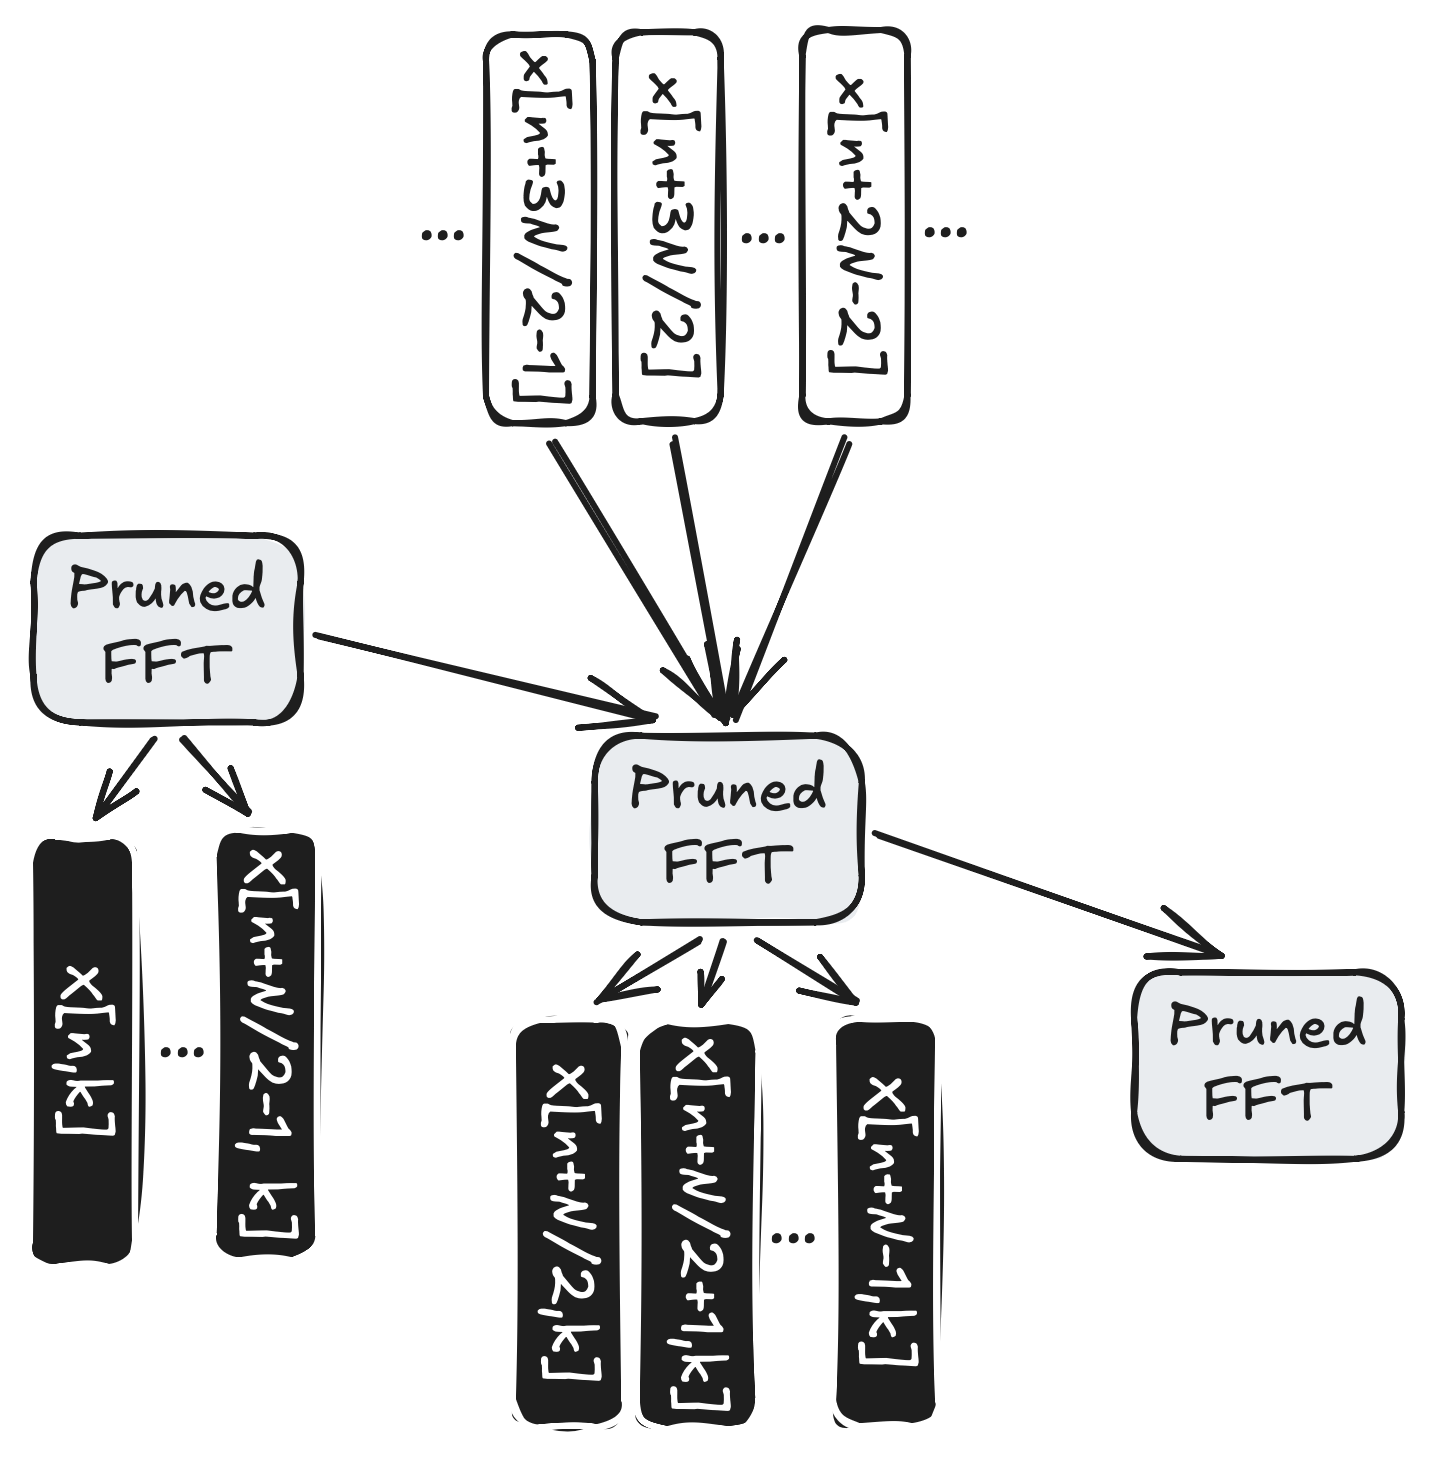
\includegraphics[width=0.5\textwidth]{figures/parallel-ff}
\end{center}

\note[item]{The serial feedforward STFT algorithm described previously cannot be
parallelized without modification. Since we are relying on the previous FFT
butterfly to compute the current one, parallelization is out of the question.}
\note[item]{To address this gap, Labao et al. proposed a quasi-parallel algorithm of 
feedforward STFT algorithm, which uses three buffers: one to store the even
and odd terms and two buffers for previous computations. By expanding the
buffers to store more computations, we can compute the next N/2 butterflies in
parallel instead of a single one like in the serial version.}
\note[item]{Shared-memory: With OpenMP, the routine in which N/2 Fourier
transforms are computed using temporary input buffer can be parallelized.}
\note[item]{Distributed-memory: N/2 Fourier transforms are as evenly distributed
as possible across all processes. Each process has its own copy of buffers, 
computes the Fourier transforms it is responsible for then writes the result 
in a local copy. All processes then do a gathering operation in which each 
sends its results to every remaining process, which allows all of them to 
correctly update their local buffers.}
\end{frame}

\begin{frame}
\frametitle{How are they compared?}
\begin{itemize}
    \item Input data are self-generated double precision arrays. 
    \item Profiling uses Linaro MAP with an input of signal size $2^{20}$ and
    window size $2^{11}$ and with 8 processes and/or 40 threads.
    \item Scaling analysis records runtime and memory usage. Time is measured by
    GNU \texttt{time}, and memory is measured as Resident Set Size by
    \texttt{ps}. Execution is done with $2^0$ to $2^7$ threads and/or $2^0$ to 
    $2^3$ processes. Data are averaged over 5 runs.
        \begin{itemize}
            \item Strong scaling uses fixed input data.
            \item Weak scaling features two settings: (1) increasing number of
            Fourier transforms and (2) increasing window size.
        \end{itemize}
\end{itemize}
\end{frame}

\begin{frame}
\frametitle{Where are they evaluated?}
\begin{itemize}
    \item Trillium cluster: 241,056 CPU cores, NDR InfiniBand 1:1 interconnect
    at 400 Gb/s, 34 PFLOPS of theoretical peak performance
    \item Niagara/Teach cluster: 2,560 CPU cores, EDR Infiniband Dragonfly+, 6
    PFLOPS of theoretical peak performance \footcite{scinet-niagara}
\end{itemize}
\begin{center}
    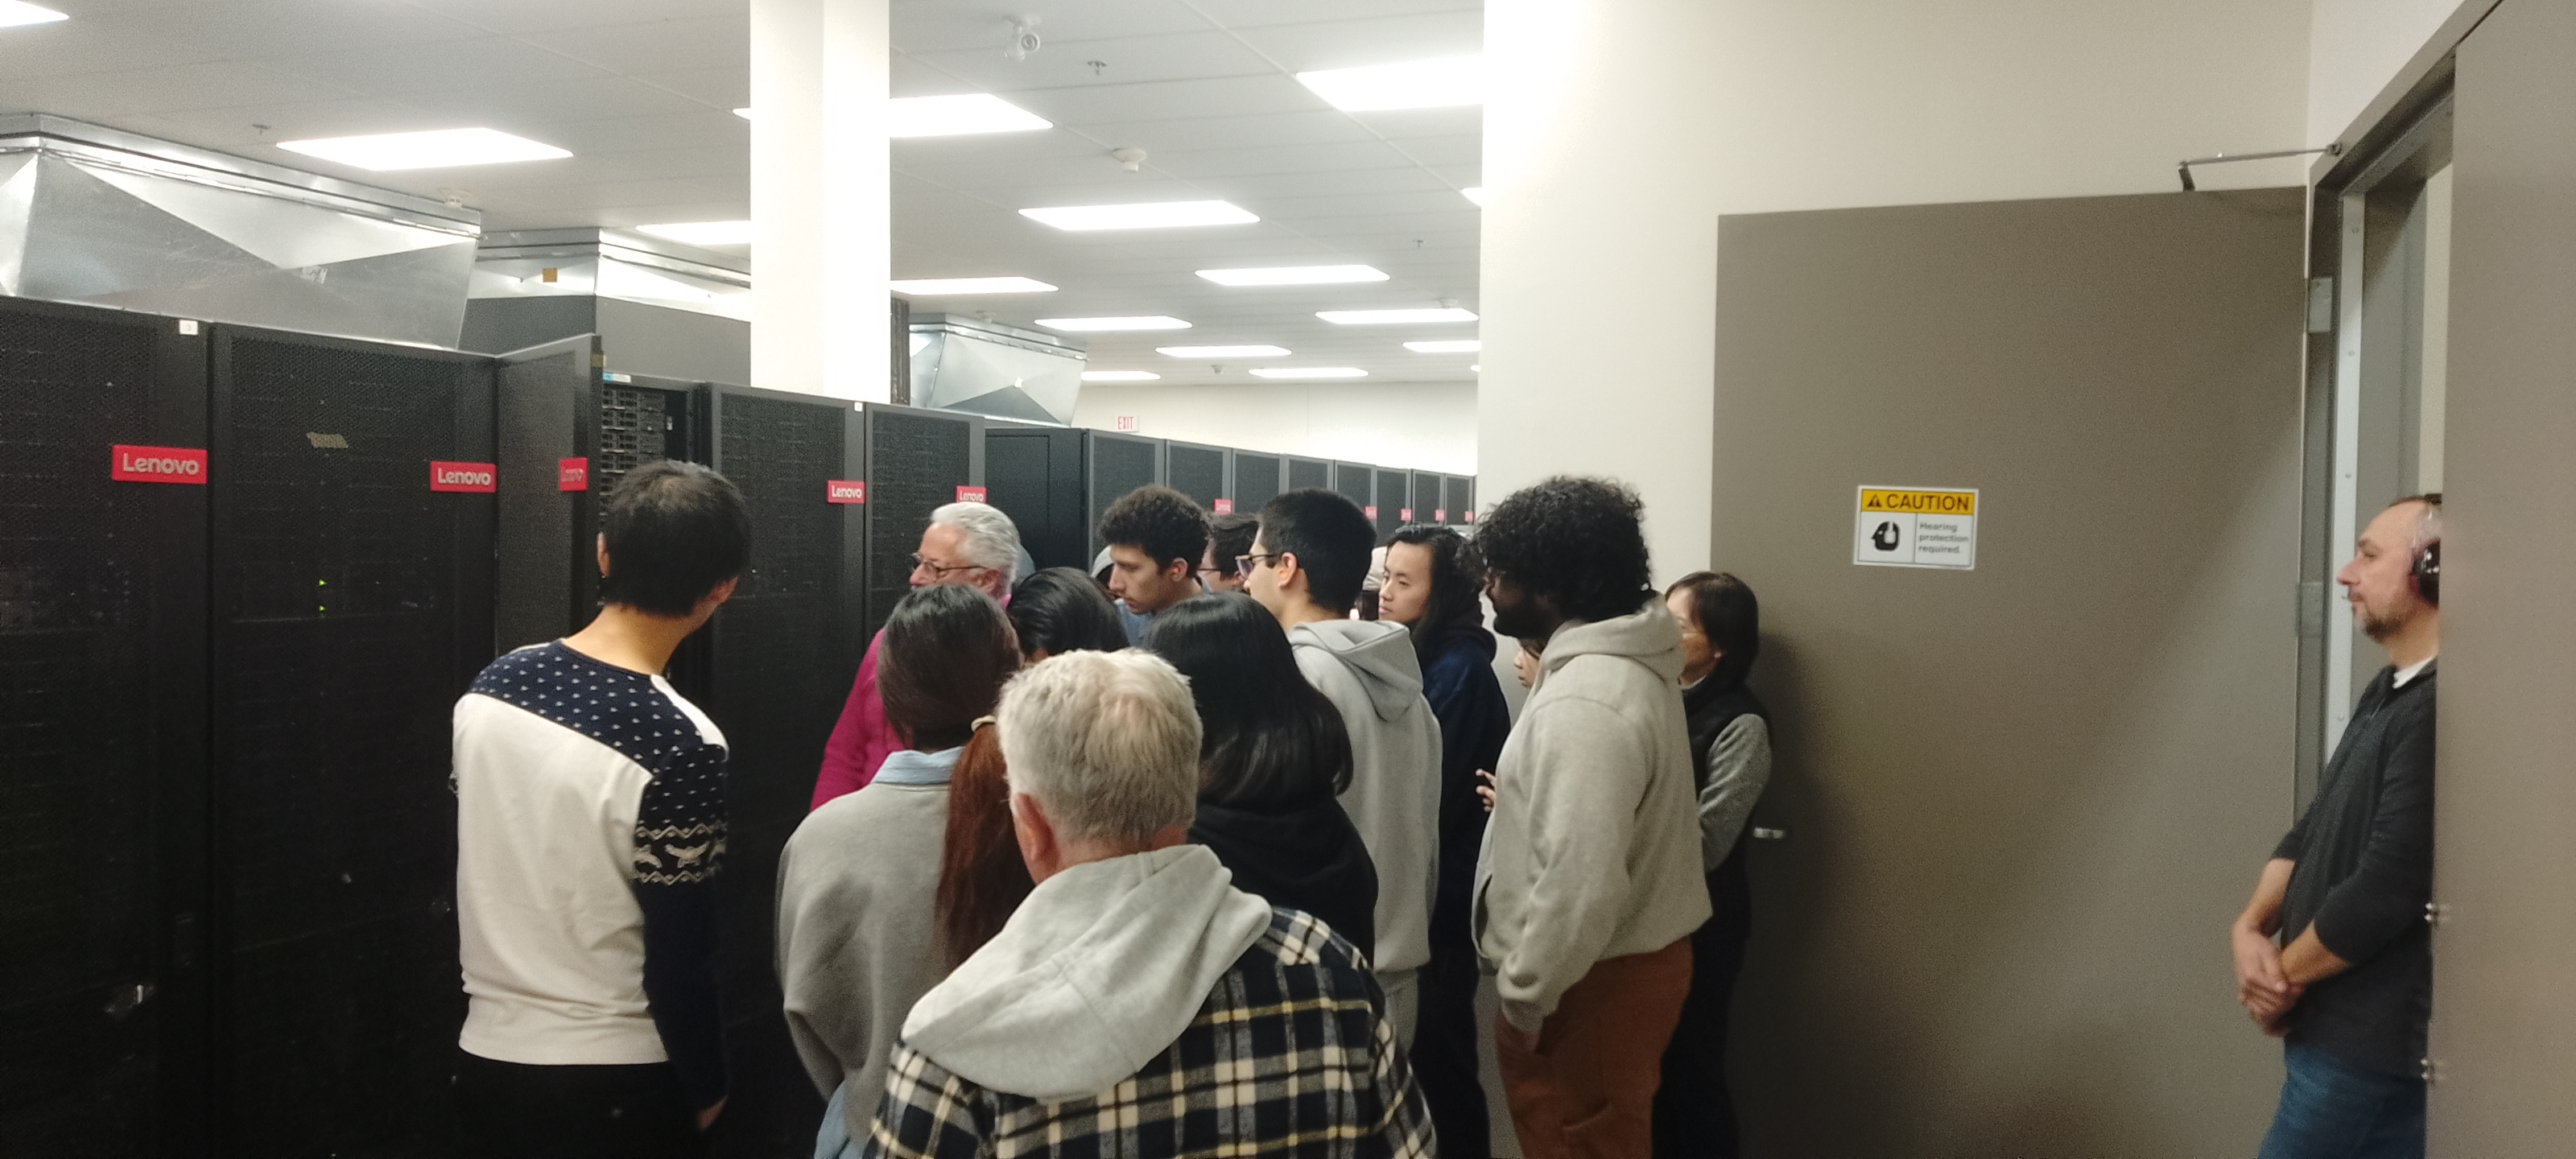
\includegraphics[width=0.8\textwidth]{figures/IMG_4308.JPG}
\end{center}
\end{frame}

\section{Results}
\begin{frame}
\frametitle{What do we find?}
\begin{itemize}
    \item Runtime of FFT-based versus feedforward algorithms
    \item Runtime variance of FFT-based versus feedforward algorithms
    \item Speedup of FFT-based versus feedforward algorithms and shared-memory
    versus distributed-memory parallel
    \item Memory usage of FFT-based versus feedforward algorithms
    \item Trillium versus Niagara/Teach clusters
\end{itemize}
\end{frame}

\begin{frame}
\frametitle{Runtime of FFT-based versus feedforward algorithms}
The feedforward algorithm is faster for lower thread/process count but slower
for higher thread/process count compared to the FFT-based algorithm.

\begin{center}
    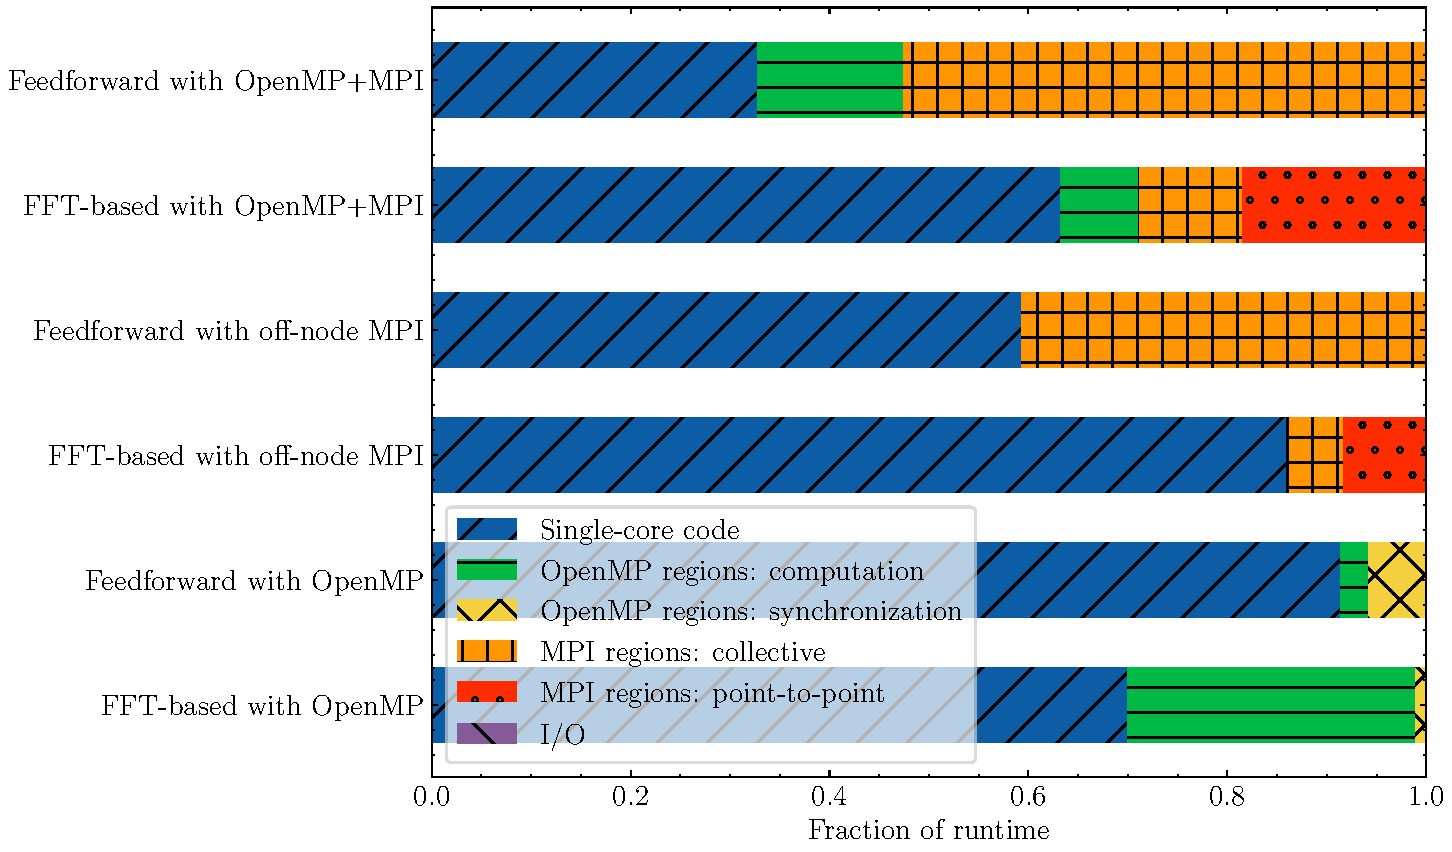
\includegraphics[width=\textwidth]{figures/profiling_time_breakdown}
\end{center}

\note[item]{The better runtime observed at smaller parallel units for the feedforward
approach is consistent with the fact that its theoretical time complexity is
better than that of the FFT-based algorithm. However, at higher
thread and process counts, the cost of synchronization incurred rises and 
offsets this slight runtime advantage.}
\note[item]{The FFT-based algorithm spends more time 
in OpenMP, most of which is for computation (96.5\%), while the OpenMP regions 
of the feedforward algorithm is dominated by synchronizationi (67.3\%). A similar
explanation can be extended for the distributed-memory configurations: the
majority of MPI regions in the FFT-based algorithm is point-to-point calls
as opposed to collective calls in the feedforward algorithm.}
\end{frame}

\begin{frame}
\frametitle{Runtime variance of FFT-based versus feedforward algorithms}
The feedforward algorithm has higher variation in runtime compared to the
FFT-based algorithm, and variation is especially large for the feedforward 
algorithm with multiprocessing.
\begin{center}
    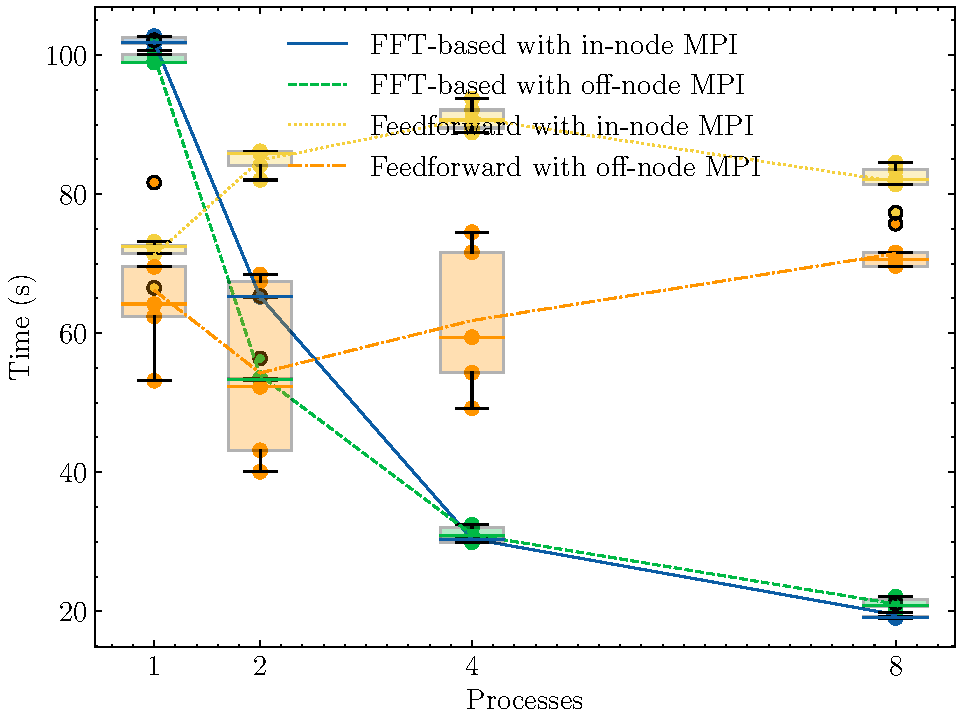
\includegraphics[width=.45\textwidth]{figures/trillium/01-mpi.pdf}\hfill
    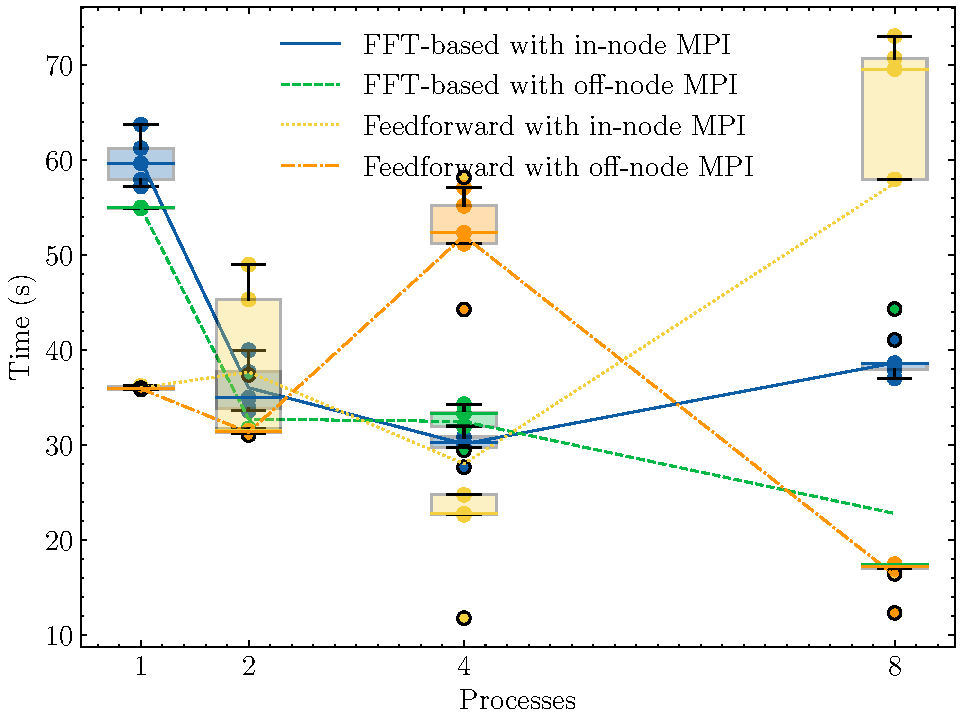
\includegraphics[width=.45\textwidth]{figures/niagara/01-mpi.pdf}\hfill
\end{center}

\note[item]{The feedforward algorithm needs to orchestrate communication for every
stage of a FFT computation while the FFT-based one only
communicates once when all parallel units finish their computation. In addition,
the communication in multiprocessing feedforward implementation is between every
process and every remaining process.}
\end{frame}

\begin{frame}
\frametitle{Speedup of FFT-based versus feedforward algorithms and shared-memory
    versus distributed-memory parallel}
    In both strong scaling and weak scaling, FFT-based algorithm outperforms
    feedforward algorithm, and MPI outperforms OpenMP with respect to speedup.
\begin{center}
    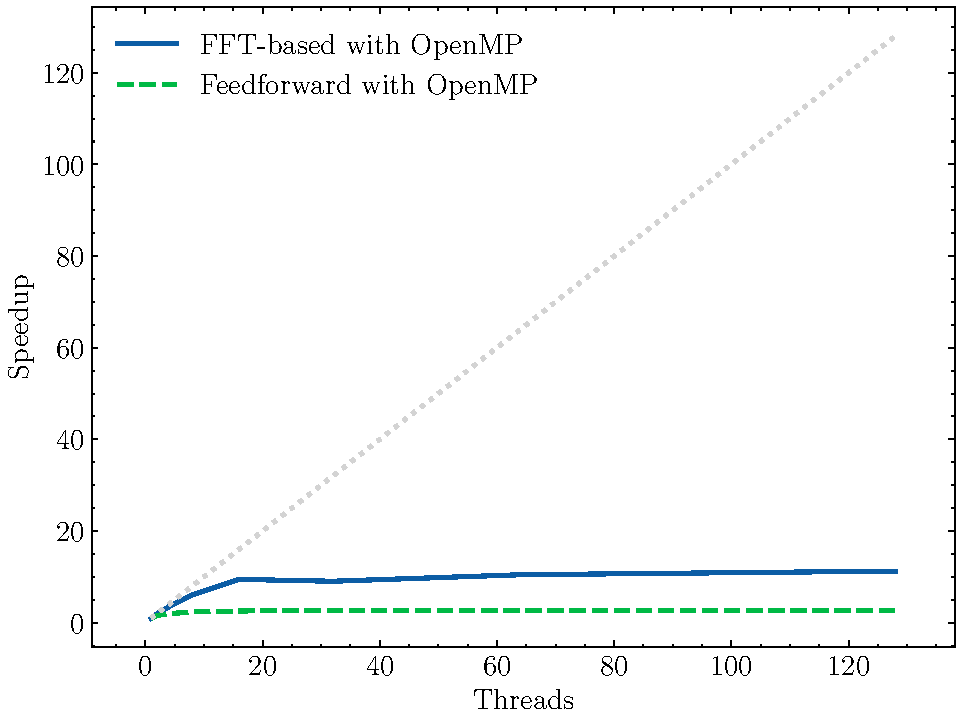
\includegraphics[width=.4\textwidth]{figures/trillium/03-ss-omp.pdf}\hfill
    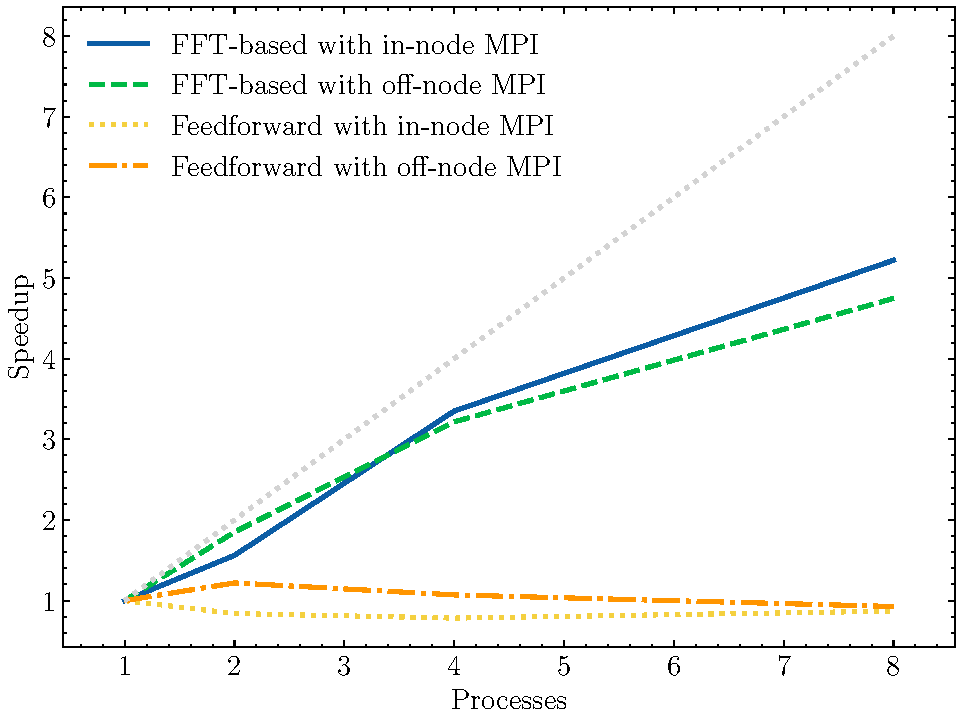
\includegraphics[width=.4\textwidth]{figures/trillium/03-ss-mpi.pdf}\hfill
    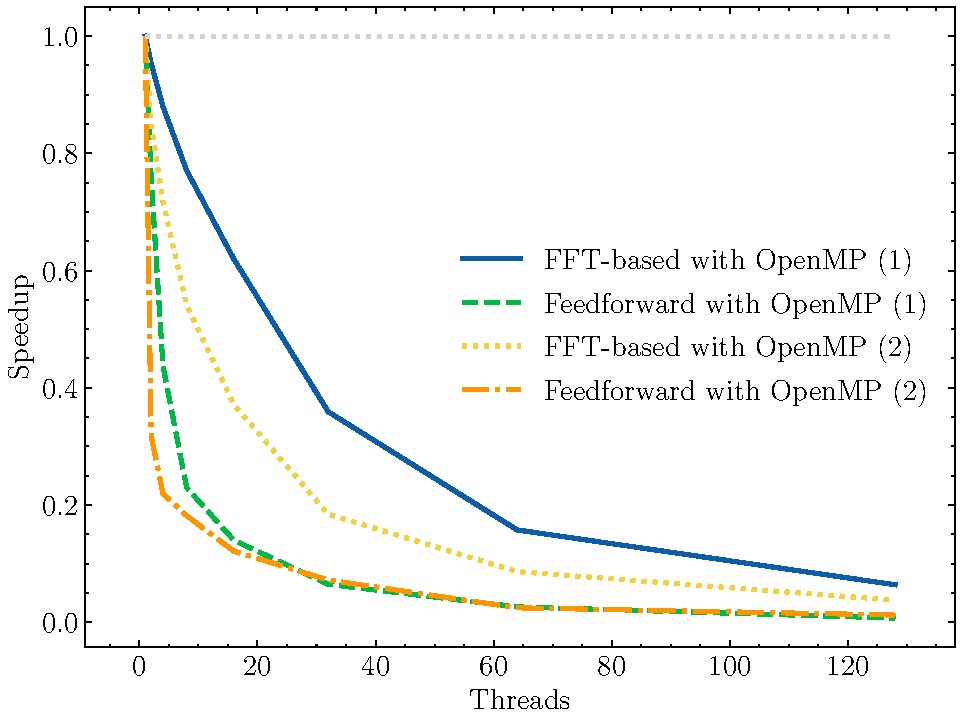
\includegraphics[width=.4\textwidth]{figures/trillium/03-ws-omp.pdf}\hfill
    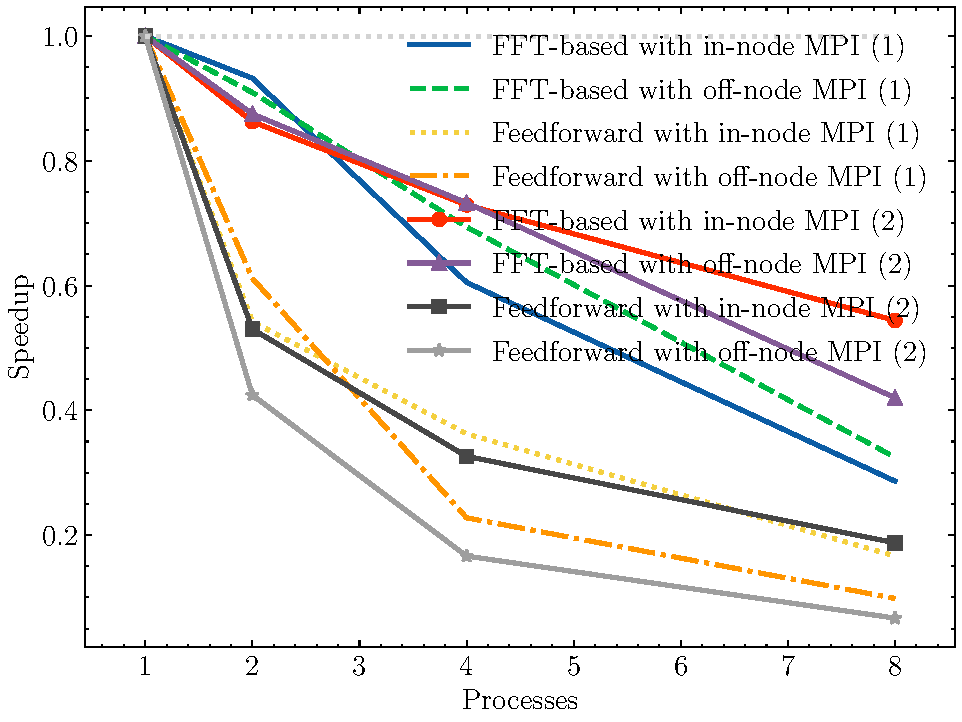
\includegraphics[width=.4\textwidth]{figures/trillium/03-ws-mpi.pdf}\hfill
\end{center}

\note[item]{The FFT-based algorithm has a higher portion of parallelizable region
as each FFT routine is done independent of one another while
the feedforward algorithm has more serial regions in which buffers are updated
and computations are reused, and thus, dependent on the previous iteration.}
\end{frame}

\begin{frame}
\frametitle{Memory usage of FFT-based versus feedforward algorithms}
Peak memory usage of the feedforward algorithm is higher than that of the
FFT-based algorithm, and peak memory usage of the MPI version is higher than
that of the OpenMP version.
\begin{center}
    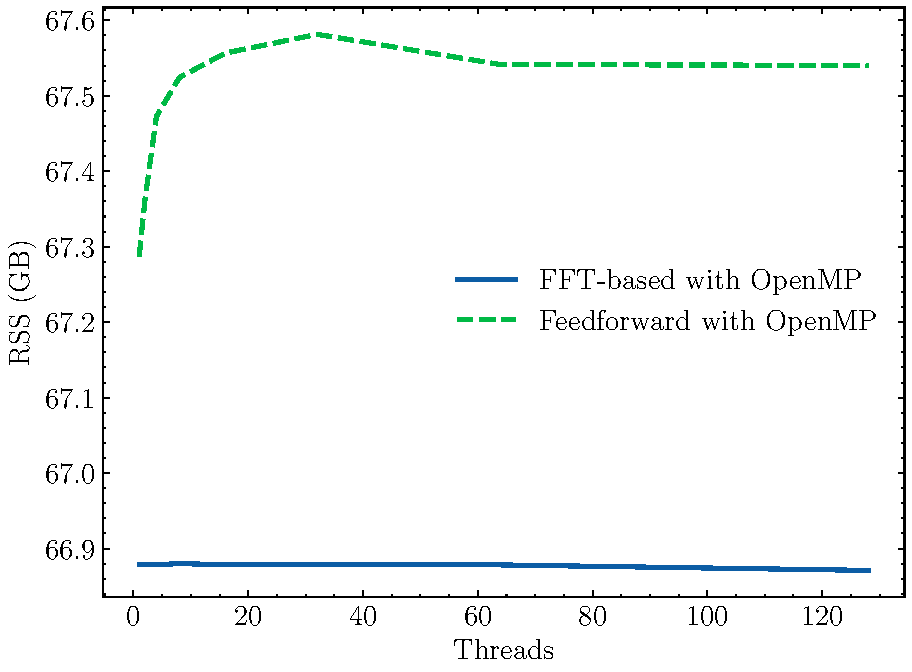
\includegraphics[width=.4\textwidth]{figures/trillium/04-ss-omp.pdf}\hfill
    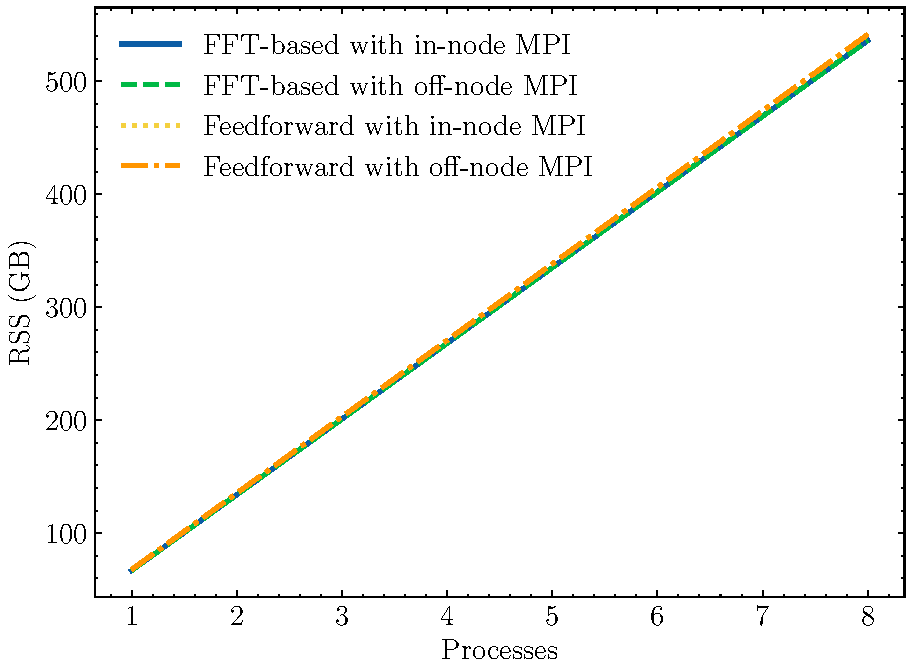
\includegraphics[width=.4\textwidth]{figures/trillium/04-ss-mpi.pdf}\hfill
    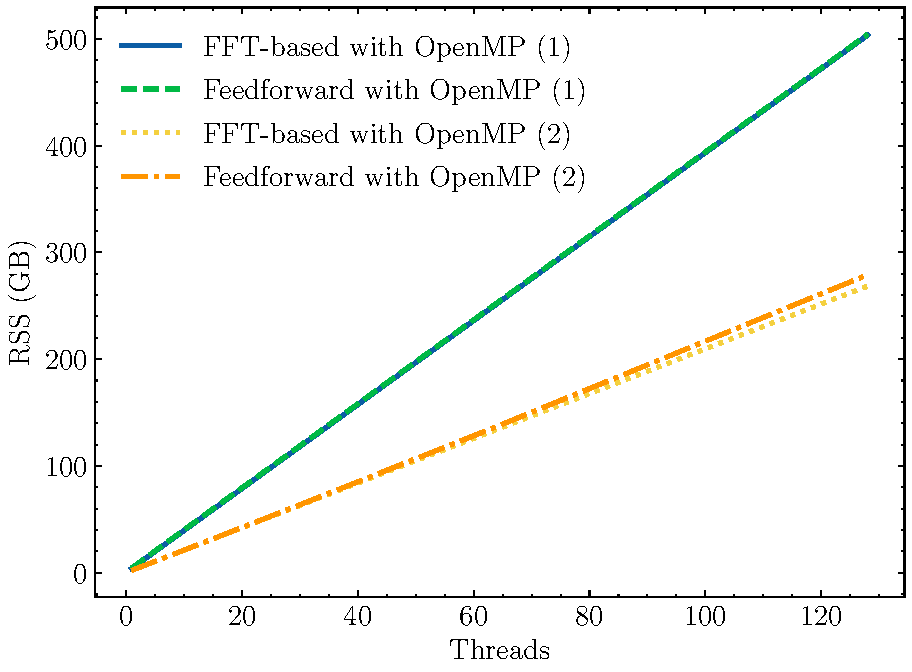
\includegraphics[width=.4\textwidth]{figures/trillium/04-ws-omp.pdf}\hfill
    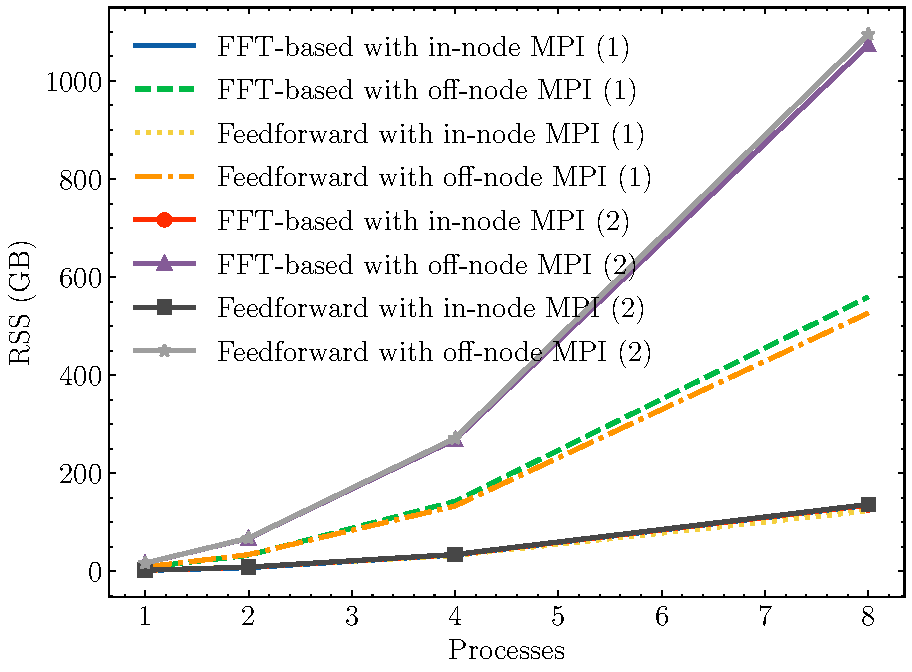
\includegraphics[width=.4\textwidth]{figures/trillium/04-ws-mpi.pdf}\hfill
\end{center}

\note[item]{Feedforward uses more memory to store previous computations.}
\note[item]{MPI uses more memory as each process has local copies of the buffers.}
\end{frame}

\begin{frame}
\frametitle{Trillium versus Niagara/Teach clusters}
All runs on Trillium cluster are faster than on Niagara/Teach cluster, but
similar patterns are observed in both.
\begin{center}
    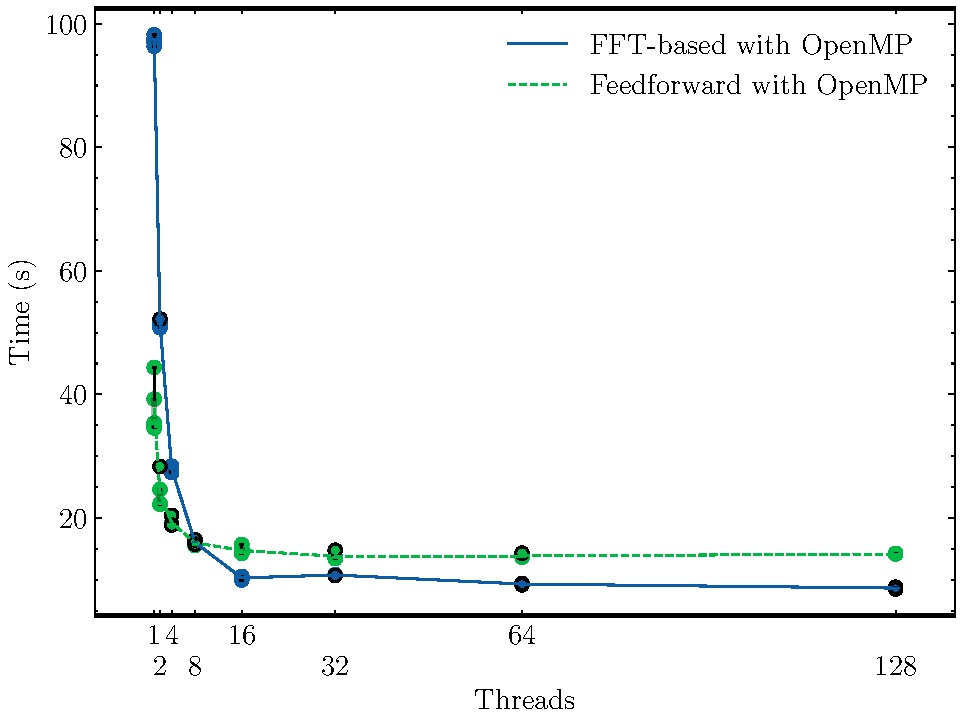
\includegraphics[width=.45\textwidth]{figures/trillium/01-omp.pdf}\hfill
    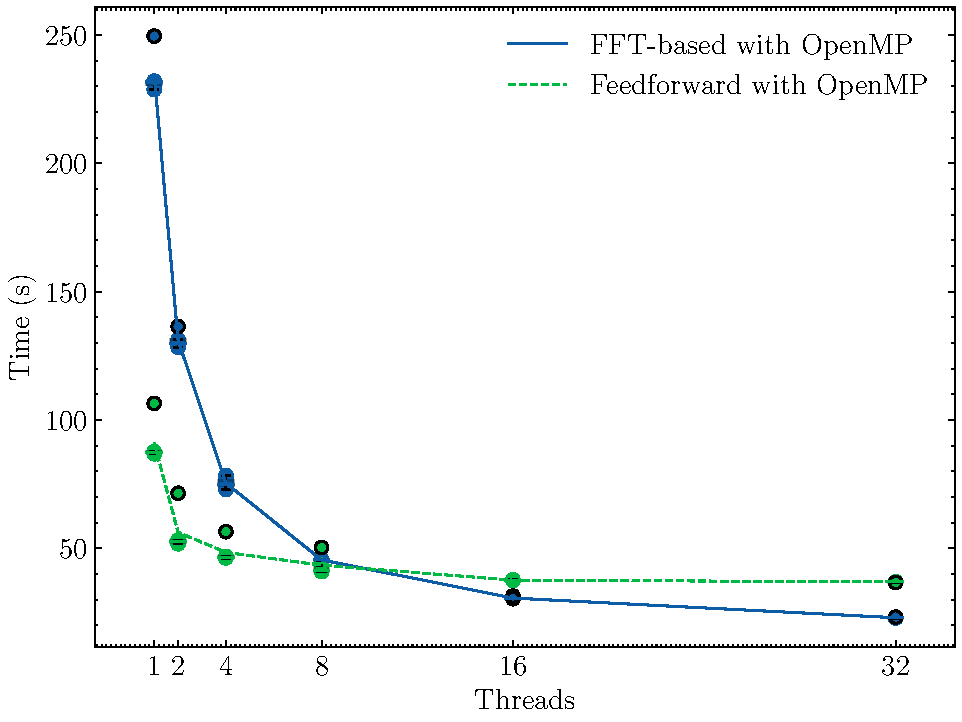
\includegraphics[width=.45\textwidth]{figures/niagara/01-omp.pdf}\hfill
\end{center}
\end{frame}

\section{Conclusion}
\begin{frame}
\frametitle{Summary}
\begin{itemize}
    \item The short-time Fourier transform reveals time-dependent information
    about the constituent frequencies of an input signal, which has many
    applications for non-stationary signals. However, its practical
    implementations are limited in approach and parallelization techniques.
    \item The FFT-based algorithm to compute STFT applies FFT to each subarray
    of the input signal, which induces redundant computations for overlapping
    segments. The feedforward algorithm only computes the new operations
    required moving from one segment to the next.
    \item A comparative analysis shows that the feedforward algorithm has better
    runtime at smaller parallel unit counts but the FFT-based algorithm has
    better efficiency. Memory usage and runtime variance are higher in the 
    feedforward algorithm. Shared-memory parallelization has closer to ideal
    speedup compared to distributed-memory.
\end{itemize}
\end{frame}

\begin{frame}
\frametitle{How can we improve?}
\begin{itemize}
    \item Extension to handle arbitrary window function, hop size, and window size
    \item Resolution for integer overflow in MPI calls
\end{itemize}

\note[item]{The implementations in this paper have several limitations. First, they assume a
rectangular window function and a hop size of 1. Second, the window size must
be a power of two. The FFT-based algorithm can generally be extended to overcome
these shortcomings. A frequency decomposing variant of the
feedforward approach by Garrido has been proposed to allow arbitrary hop 
sizes and different window functions.}
\note[item]{The multiprocessing implementation of the feedforward algorithm has been tested
with window size up to 2 to 18, but larger window size will crash the program
due to integer overflow in MPI calls. This problem may be resolved by slicing 
the data to be communicated, but this approach can potentially cause unbalanced 
workload. Another solution is to use MPI-4 support for large datatypes and
procedures that work with these large types to increase the limit of the window
size; however, this was not tested as part of this study as MPI-4 was not
available on the clusters used at the moment of completing our work.}
\end{frame}

\begin{frame}[t, allowframebreaks]
\frametitle{References}
\printbibliography[heading=none]
\end{frame}

\end{document}
